\documentclass[10pt,letterpaper,journal]{IEEEtran}
\usepackage{cite}
\usepackage{url}
\usepackage{graphicx}
\usepackage{booktabs}
\usepackage{pifont}
\usepackage{amssymb}
\usepackage{xcolor}
\usepackage{array}
\usepackage{tabularx}
\usepackage{amsmath}
\usepackage{amsthm}
\usepackage{newtxtext}
\usepackage{enumitem}
\usepackage{stfloats}
\usepackage{subcaption}
\usepackage{microtype}
\usepackage{tikz}
\usetikzlibrary{arrows.meta}

\title{Constraint-Aware Zero-Knowledge Face Eligibility Against Lookalike Attackers: Sound Circuits and Attested Capture for Decentralized Voting}

\author{\IEEEauthorblockN{Mahin R. Chowdhury\IEEEauthorrefmark{1}\IEEEmembership{Student Member, IEEE},
K.~M.~Azharul Hasan\IEEEauthorrefmark{1}\IEEEmembership{Member, IEEE},
Arpita Das\IEEEauthorrefmark{1}\IEEEmembership{Student Member, IEEE}}\\
\IEEEauthorblockA{\IEEEauthorrefmark{1}Department of Computer Science and Engineering,\\
Khulna University of Engineering \& Technology,\\
Khulna-9203, Bangladesh\\
}}

%\IEEEpubid{0000--0000/00\$00.00~\copyright~2026 IEEE}

\markboth{IEEE Transactions on Information Forensics and Security,~Vol.~XX, No.~XX, Month~2026}{Chowdhury \emph{et al.}: Constraint-Aware Zero-Knowledge Face Eligibility}

\newcommand{\vect}[1]{\mathbf{#1}}
% Generated by make_numbers.py from api-server/{benchmark,results}/*.json. Do not edit.
\newcommand{\nDim}{128}
\newcommand{\nTau}{0.35}
\newcommand{\nTauNum}{1{,}225}
\newcommand{\nLfwEer}{0.22}
\newcommand{\nLfwEerLo}{0.13}
\newcommand{\nLfwEerHi}{0.32}
\newcommand{\nFrr}{0.60}
\newcommand{\nFar}{0.013}
\newcommand{\nFalseAccepts}{26}
\newcommand{\nImpostorPairs}{200{,}000}
\newcommand{\nFacenetEer}{4.38}
\newcommand{\nFacenetEerLo}{4.02}
\newcommand{\nFacenetEerHi}{4.78}
\newcommand{\nCelebaEer}{4.02}
\newcommand{\nCelebaEerLo}{3.55}
\newcommand{\nCelebaEerHi}{4.49}
\newcommand{\nCelebaEmbedded}{39{,}726}
\newcommand{\nCelebaImages}{39{,}733}
\newcommand{\nMaleEer}{2.25}
\newcommand{\nMaleEerLo}{1.92}
\newcommand{\nMaleEerHi}{2.59}
\newcommand{\nFemaleEer}{5.10}
\newcommand{\nFemaleEerLo}{4.67}
\newcommand{\nFemaleEerHi}{5.69}
\newcommand{\nMaleIds}{878}
\newcommand{\nFemaleIds}{1{,}122}
\newcommand{\nGenderGap}{2.8}
\newcommand{\nGenderRatio}{2.3}
\newcommand{\nCelebaRawEer}{3.59}
\newcommand{\nFacenetCelebaEer}{8.09}
\newcommand{\nFacenetMaleEer}{7.93}
\newcommand{\nFacenetFemaleEer}{10.47}
\newcommand{\nDeepfaceEer}{6.10}
\newcommand{\nDeepfaceRatio}{46}
\newcommand{\nRawEer}{0.13}
\newcommand{\nInvCos}{0.72}
\newcommand{\nInvEer}{0.27}
\newcommand{\nInvRawEer}{0.13}
\newcommand{\nCalfwEer}{6.70}
\newcommand{\nCalfwEerLo}{5.88}
\newcommand{\nCalfwEerHi}{7.48}
\newcommand{\nCalfwRawEer}{6.47}
\newcommand{\nCalfwFrr}{9.6}
\newcommand{\nCalfwFar}{0.13}
\newcommand{\nCalfwUnseenFrr}{9.5}
\newcommand{\nCalfwImages}{7{,}156}
\newcommand{\nCalfwEmbedded}{7{,}156}
\newcommand{\nCplfwEer}{5.56}
\newcommand{\nCplfwEerLo}{4.93}
\newcommand{\nCplfwEerHi}{6.23}
\newcommand{\nCplfwRawEer}{4.65}
\newcommand{\nCplfwFrr}{13.8}
\newcommand{\nCplfwFar}{0.24}
\newcommand{\nCplfwUnseenFrr}{14.3}
\newcommand{\nCplfwImages}{5{,}984}
\newcommand{\nCplfwEmbedded}{5{,}950}
\newcommand{\nLookLfwOne}{0.004}
\newcommand{\nLookLfwTen}{0.10}
\newcommand{\nLookLfwHundred}{0.85}
\newcommand{\nLookLfwThousand}{8.4}
\newcommand{\nLookCelebaOne}{0.01}
\newcommand{\nLookCelebaTen}{0.16}
\newcommand{\nLookCelebaHundred}{1.7}
\newcommand{\nLookCelebaThousand}{14.1}
\newcommand{\nLookGenderOne}{0.03}
\newcommand{\nLookGenderTen}{0.21}
\newcommand{\nLookGenderHundred}{2.3}
\newcommand{\nLookGenderThousand}{25.6}
\newcommand{\nZeLookLfwOne}{0.10}
\newcommand{\nZeLookLfwTen}{0.97}
\newcommand{\nZeLookLfwHundred}{9.0}
\newcommand{\nZeLookLfwThousand}{59.6}
\newcommand{\nZeLookCelebaOne}{0.16}
\newcommand{\nZeLookCelebaTen}{1.4}
\newcommand{\nZeLookCelebaHundred}{13.3}
\newcommand{\nZeLookCelebaThousand}{71.1}
\newcommand{\nZeLookGenderOne}{0.20}
\newcommand{\nZeLookGenderTen}{1.8}
\newcommand{\nZeLookGenderHundred}{16.0}
\newcommand{\nZeLookGenderThousand}{83.7}
\newcommand{\nZeFrr}{0.47}
\newcommand{\nFaceConstraints}{32{,}668}
\newcommand{\nIrisConstraints}{17{,}518}
\newcommand{\nHashConstraints}{7{,}041}
\newcommand{\nCosConstraints}{5{,}656}
\newcommand{\nEuclidConstraints}{5{,}296}
\newcommand{\nMerkleConstraints}{4{,}840}
\newcommand{\nAttestConstraints}{7{,}368}
\newcommand{\nKeyMB}{30.9}
\newcommand{\nIrisKeyMB}{14.2}
\newcommand{\nAttestShare}{23}
\newcommand{\nPoseidonTwo}{240}
\newcommand{\nPackedHash}{1{,}905}
\newcommand{\nHamming}{778}
\newcommand{\nSigma}{5 \times 10^{5}}
\newcommand{\nCoordBits}{19}
\newcommand{\nTwoCoordBits}{38}
\newcommand{\nRangePerCoord}{20}
\newcommand{\nRangeConstraints}{5{,}120}
\newcommand{\nDotBits}{45}
\newcommand{\nCmpBits}{104}
\newcommand{\nDomainExp}{15}
\newcommand{\nHashSixteen}{1{,}044}
\newcommand{\nCosSixteen}{831}
\newcommand{\nFullCosSixteen}{15{,}849}
\newcommand{\nHashSixtyFour}{3{,}618}
\newcommand{\nCosSixtyFour}{2{,}901}
\newcommand{\nFullCosSixtyFour}{23{,}067}
\newcommand{\nHashNinetySix}{5{,}328}
\newcommand{\nCosNinetySix}{4{,}280}
\newcommand{\nFullCosNinetySix}{27{,}866}
\newcommand{\nHashOneSixty}{9{,}198}
\newcommand{\nCosOneSixty}{7{,}035}
\newcommand{\nFullCosOneSixty}{38{,}361}
\newcommand{\nHashTwoFiftySix}{14{,}322}
\newcommand{\nCosTwoFiftySix}{11{,}163}
\newcommand{\nFullCosTwoFiftySix}{52{,}737}
\newcommand{\nOneSixtyExtra}{17}
\newcommand{\nPerDim}{154}
\newcommand{\nEuclidSixtyFour}{2{,}672}
\newcommand{\nFullEuclidSixtyFour}{22{,}838}
\newcommand{\nFullEuclid}{32{,}308}
\newcommand{\nEuclidSaveSixtyFour}{229}
\newcommand{\nEuclidSave}{360}
\newcommand{\nMerkleMs}{53}
\newcommand{\nMerkleCi}{0.2}
\newcommand{\nEncryptMs}{83}
\newcommand{\nEncryptCi}{3}
\newcommand{\nWitnessMs}{209}
\newcommand{\nWitnessCi}{3}
\newcommand{\nProveMs}{1{,}345}
\newcommand{\nProveCi}{16}
\newcommand{\nClientMs}{1{,}690}
\newcommand{\nClientCi}{16}
\newcommand{\nSignMs}{27}
\newcommand{\nSignCi}{0.2}
\newcommand{\nVerifyMs}{19}
\newcommand{\nVerifyCi}{2}
\newcommand{\nCastVoteMs}{49}
\newcommand{\nCastVoteCi}{1}
\newcommand{\nProveShare}{80}
\newcommand{\nProveS}{1.35}
\newcommand{\nClientS}{1.7}
\newcommand{\nIrisProveS}{0.81}
\newcommand{\nIrisWitnessMs}{140}
\newcommand{\nIrisWitnessCi}{1}
\newcommand{\nIrisProveMs}{811}
\newcommand{\nIrisProveCi}{10}
\newcommand{\nIrisClientMs}{1{,}085}
\newcommand{\nIrisClientCi}{11}
\newcommand{\nIrisSignMs}{24}
\newcommand{\nIrisSignCi}{0.2}
\newcommand{\nIrisVerifyMs}{18}
\newcommand{\nIrisVerifyCi}{2}
\newcommand{\nIrisCastVoteMs}{49}
\newcommand{\nIrisCastVoteCi}{1}
\newcommand{\nScaleTenPathsMs}{4}
\newcommand{\nScaleTenProveMs}{1{,}368}
\newcommand{\nScaleTenCastMs}{49}
\newcommand{\nScaleThousandPathsMs}{52}
\newcommand{\nScaleThousandProveMs}{1{,}356}
\newcommand{\nScaleThousandCastMs}{49}
\newcommand{\nScaleFiveThousandPathsMs}{248}
\newcommand{\nScaleFiveThousandProveMs}{1{,}324}
\newcommand{\nScaleFiveThousandCastMs}{50}
\newcommand{\nScaleTwentyThousandPathsMs}{987}
\newcommand{\nScaleTwentyThousandProveMs}{1{,}368}
\newcommand{\nScaleTwentyThousandCastMs}{48}
\newcommand{\nScaleCastMin}{48}
\newcommand{\nScaleCastMax}{50}
\newcommand{\nScalePathsTopS}{1.0}
\newcommand{\nScalePathsMillionS}{49}
\newcommand{\nTallyVerifyMs}{27}
\newcommand{\nTallyPublishS}{0.43}
\newcommand{\nTallyMillionMin}{7}
\newcommand{\nTallyHundredVerifyS}{2.8}
\newcommand{\nTallyHundredDecryptMs}{28}
\newcommand{\nTallyHundredPublishMs}{68}
\newcommand{\nTallyThousandVerifyS}{27.4}
\newcommand{\nTallyThousandDecryptMs}{28}
\newcommand{\nTallyThousandPublishMs}{425}
\newcommand{\nFabVoters}{40}
\newcommand{\nFabInFlight}{10}
\newcommand{\nFabSeqS}{2.14}
\newcommand{\nFabConcS}{0.62}
\newcommand{\nFabTps}{16}
\newcommand{\nFabMillionH}{17}
\newcommand{\nFabRegisterS}{2.12}
\newcommand{\nFabPublishS}{2.23}
\newcommand{\nFabKeygenS}{10.4}
\newcommand{\nIrisProveShare}{75}
  % measured numbers, generated by make_numbers.py

\newtheorem{theorem}{Theorem}[section]
\newtheorem{lemma}[theorem]{Lemma}
\newtheorem{definition}[theorem]{Definition}
\newtheorem{proposition}[theorem]{Proposition}
\newtheorem{corollary}[theorem]{Corollary}
\newtheorem{remark}[theorem]{Remark}
\newtheorem{assumption}[theorem]{Assumption}

\newcommand{\cmark}{\textcolor{green!60!black}{\ding{51}}}   % checkmark
\newcommand{\pmark}{\textcolor{orange}{\textbf{$\sim$}}}      % partial
\newcommand{\xmark}{\textcolor{red}{\ding{55}}}   

% Start document
\begin{document}

\maketitle

\begin{abstract}
A zero-knowledge face match is only as sound as its weakest constraint, and the weak constraints are the ones an honest prover never exercises. We identify six such pitfalls in biometric eligibility circuits (a free live witness, a prover-chosen threshold, unconstrained Merkle path bits, missing coordinate range checks, unbound public inputs and unattested enrollment) and exploit each against a Hyperledger Fabric voting system: without its check the attack succeeds, and with the checks every attack is rejected. A generic circuit analyzer flags only one of the five pitfalls that live in the circuit. The fixes are a face-eligibility circuit that binds every live sample, and every enrolled template, to a registered capture kiosk by an in-circuit EdDSA signature that hides which ballot it enabled, and a chaincode that enforces every check and verifies a threshold tally. Soundness also shapes cost: range checks dominate the comparator, and because they bound every coordinate, packed template hashing becomes nearly free and the circuit shrinks by \nPackSave\%. A face is public, so behind a stolen credential the threshold must resist lookalikes found by screening photos; we bound such an attacker by $1-(1-\mathsf{FAR})^K$ and select, on validation identities only, a \nDim{}-D PCA of ArcFace embeddings at which screening 100 candidates succeeds \nLookLfwHundred\% of the time. Game-based security theorems are each tied to a constraint or chaincode check. A voter's browser builds a ballot in \nBrowserClientS~s, and the chaincode verifies it in \nCastVoteMs~ms regardless of electorate size.
\end{abstract}

\IEEEpubidadjcol

\begin{IEEEkeywords}
Biometrics, zero-knowledge proofs, template protection, arithmetic circuits, circuit soundness, privacy-preserving authentication, electronic voting, Groth16.
\end{IEEEkeywords}

% Main body of manuscript

% ============================================================
%  SECTION I --- INTRODUCTION 
% ============================================================

\section{Introduction}
\label{sec:intro}

A biometric ties a credential to a person, but a template exposed on a ledger or server is compromised for good, since it cannot be reissued like a key~\cite{Jain2008,Rathgeb2011}. Zero-knowledge succinct arguments (zk-SNARKs~\cite{Groth2016}) let a user prove that a live sample matches an enrolled template without revealing either.

Such circuits are easy to get subtly wrong, because the constraints that matter are the ones an honest prover never exercises. We identify six pitfalls, each exploitable against a real deployment (Table~\ref{tab:attack_suite}):
(P1)~a \emph{free live witness}: if the live sample is a private input, the proof shows knowledge of a template rather than a presented face, so a stolen credential suffices (A6, A13--A16);
(P2)~a \emph{prover-chosen threshold}: a threshold passed as a public input that the verifier does not pin makes the match vacuous (A2);
(P3)~\emph{unconstrained path bits}: circomlib's \texttt{Switcher} does not force its selector to $\{0,1\}$, so membership can be forged from any leaf (A1);
(P4)~\emph{missing range checks}: a real-valued comparator over $\mathbb{F}_p$ is sound only if no product wraps modulo $p$ and the sign survives squaring (A5), and a packed template hash aliases without them (A24);
(P5)~\emph{unbound public inputs}: an election identifier or ciphertext the verifier does not recompute permits re-voting and front-running (A3, A7), and a public template hash links every ballot (A4);
(P6)~\emph{unattested enrollment}: a commitment the registrar cannot inspect may encode someone else's face (A25--A27).
As specified, zkSABER~\cite{zkSABER2025}, the closest prior design, exhibits P1, P2 and P4, and its nullifier is not unique per credential (\S\ref{sec:related}). Soundness also sets the cost: range checks take \nRangePerCoord{} constraints per coordinate and dominate the comparator, but once paid for they make packing the template injective, so hashing it costs almost nothing. Finally, a face is public: behind a stolen credential, a zero-effort false-accept rate understates an attacker who screens photos offline for a lookalike.

Why biometrics, kiosks and a ledger? An anonymous credential alone, as in Semaphore~\cite{Gurkan2020}, is a bearer token: it can be sold, lent or stolen, and nothing ties a ballot to the person enrolled. In-person voting closes that gap by having staff check identity and mark a roll, so eligibility is auditable only by trusting that staff. Here a supervised kiosk captures the face but learns neither the credential nor the ballot, the proof ties every counted ballot to an enrolled credential and to a matching live capture, and anyone can check this on a ledger that several organizations maintain, so no single operator controls the bulletin board. The registration authority and the kiosk registry remain trusted for eligibility (\S\ref{sec:system_model}).

This paper presents a sound zero-knowledge face-verification circuit for anonymous eligibility, and deploys it in a voting system in which voters prove, encrypt and sign on their own devices. The evaluation answers three research questions:
\textbf{RQ1}: what does a \emph{sound} biometric comparator cost in-circuit, and which encoding minimizes that cost without losing accuracy?
\textbf{RQ2}: what does casting a ballot cost the voter's device and the ledger, and how does it scale with the electorate?
\textbf{RQ3}: can every check be enforced on-chain, so that the gateway need not be trusted, and at what cost?

\noindent\textbf{Key Contributions.}
\begin{enumerate}[leftmargin=*,noitemsep,topsep=1pt,parsep=0pt]
    \item \textbf{Six Soundness Pitfalls, Each Exploited:} an attack suite against the production circuits and chaincode turns every pitfall, and every premise of the security theorems, into a concrete witness or transaction that succeeds without its check and is rejected with it (Table~\ref{tab:attack_suite}). On variants of our circuit with one fix removed each, the Circomspect analyzer flags only P5.
    \item \textbf{Attested Capture and Enrollment:} the live sample is bound in-circuit to a registered capture device by an EdDSA signature over the sample, the election and a hiding commitment to the nullifier, so the proof shows that a registered device captured the sample (liveness rests on the device's PAD) without the device learning which ballot it enabled; enrollment is attested the same way, so the RA need not trust that a client's commitment encodes the enrollee's face (Section~\ref{sec:protocol_construction}).
    \item \textbf{Soundness-Aware Packing and Lookalike-Aware Encoding:} because the range checks bound every coordinate, the template packs twelve coordinates per field element, so hashing it is nearly free and the circuit shrinks by \nPackSave\%. A $K$-screening game bounds a lookalike attacker by $1-(1-\mathsf{FAR})^K$; against $K = 100$, a rule applied to validation identities only selects PCA-128 at $\tau = 0.35$ (on test pairs, \nLookLfwHundred\% lookalike success at \nFrr\% FRR), half the circuit of raw 512-D ArcFace, where the usual zero-effort rule would have deployed 96-D, which that attacker beats \nZeLookLfwHundred\% of the time. A circuit-specific discriminant projection (SOPQ) is a negative result.
    \item \textbf{Security and Evaluation:} game-based eligibility, one-vote, integrity, privacy and verifiability theorems whose every premise is a constraint or chaincode check, with a $t$-of-$n$ key the chaincode derives from a Pedersen DKG~\cite{Pedersen1991} and a tally it verifies itself (Section~\ref{sec:security}); LFW~\cite{Huang2007LFW} and CelebA~\cite{Liu2015CelebA} accuracy with bootstrap CIs, cross-age and cross-pose rejection (\nCalfwFrr\% and \nCplfwFrr\% FRR), a gender gap (\nMaleEer\% vs.\ \nFemaleEer\% EER), template inversion, proving in a real browser, and a 40-voter election on a live two-organization Fabric network. An iris variant is near chance under classical segmentation and is reported only in Supplementary Material, Appendix~D.
\end{enumerate}

\section{Related Work}
\label{sec:related}


\subsection{Biometric Template Protection and Cancelable Biometrics}
\label{subsec:rel_biometric}
Protecting stored biometric references against compromise is central to biometric security. Foundational approaches include fuzzy commitments~\cite{JuelsWattenberg1999} and fuzzy extractors~\cite{Dodis2004}, which bind error-correcting codewords to noisy biometric vectors, and cancelable biometrics~\cite{Rathgeb2011}, which apply non-invertible transforms to templates at the cost of accuracy and residual linkage-attack vulnerability across compromised databases.
Our evaluated SOPQ projection (discriminant, then orthonormalized) is related to linear discriminant analysis and to Iterative Quantization (ITQ)~\cite{Gong2013}, which learns an orthogonal rotation minimizing quantization error for binary hashing. Neither treats R1CS constraint count as a design objective, which we do (Section~\ref{sec:metric_formulation}).

Recent work applies zero-knowledge and multi-party primitives to biometrics: Mao et al.~\cite{Mao2023} prove Euclidean distance with a commitment-based ZK protocol, Guo et al.~\cite{Guo2024} integrate commitments with verifiable classifiers, Blanton et al.~\cite{Blanton2024} evaluate private fingerprint matching via garbled circuits, and ledger-anchored identity appears in BioZero~\cite{Lai2024}, Mao et al.~\cite{Mao2025}, and ZK-SERIES~\cite{ZKSeries2025}; World~ID checks iris-code uniqueness in multi-party computation~\cite{WorldID2024}, and its zero-knowledge proof covers membership of a registered secret, not the biometric. These predominantly rely on proprietary hardware oracles or lack formal security proofs.
The closest prior work is zkSABER~\cite{zkSABER2025}, which proves in one Groth16 circuit Merkle membership, a nullifier, and a quantized cosine match of face embeddings, with constant on-chain cost. As specified, its threshold $\tau'$ is part of the public statement and is not pinned by the contract, its nullifier $\mathcal{H}(\omega_{sk}, r)$ takes a prover-chosen $r$, so it is not unique per credential, and the live embedding is a free witness with no stated range check or capture attestation. These are the checks that our attacks A2, A3, A5 and A6 show to be necessary (Table~\ref{tab:attack_suite}); we did not run them against zkSABER. FHE permits distance evaluation over ciphertexts, but at a far higher computational cost than plaintext matching~\cite{Karakosta2025}, which makes client-side zk-SNARK proving the more practical choice for voters proving on commodity endpoints.

\subsection{Arithmetic Circuit Complexity and Zero-Knowledge Systems}
\label{subsec:rel_circuit}
In zero-knowledge proof systems such as Groth16~\cite{Groth2016}, PLONK, and STARKs, the comparison metric's arithmetic structure governs circuit complexity: computation is expressed over $\mathbb{F}_p$ as an R1CS, where linear combinations are near-free but non-linear multiplications dictate constraint counts and memory footprint.
Daugman's IrisCode~\cite{Daugman2004,Daugman2016} evaluates Hamming distance via linear bitwise constraints ($\text{xor}_j = a_j + b_j - 2a_j b_j$), one multiplication and one Boolean check per bit, scaling as $\mathcal{O}(d)$. Continuous facial embeddings (128- to 512-D) instead need cosine or Euclidean metrics (inner products, norms and a cross-multiplied threshold), still $\mathcal{O}(d)$ multiplications but with per-coordinate range checks for soundness. Benchmarking studies survey general ZK proof engines~\cite{OudeRoelink2024}, but we know of no prior work that chooses a biometric encoding by its measured, soundness-inclusive circuit cost.
Under-constrained circuits are the dominant class of SNARK vulnerabilities~\cite{Chaliasos2024SoK}, and tools detect them automatically~\cite{Pailoor2023,Wen2024ZKAP}. Our P3, P4 and the unchecked-input part of P5 are instances of these known classes; P1, P2, P6 and the packing alias are specific to biometric statements: the circuit is well formed, but the statement it proves is too weak. On variants of our circuit with exactly one fix removed each, Circomspect~\cite{Circomspect} flags only P5 (an unused public input and an unchecked nullifier) and reports nothing new for P1--P4; P6 is not a property of the vote circuit at all.

\subsection{Decentralized Authentication and E2EV Case Studies}
\label{subsec:rel_e2ev}
Decentralized end-to-end verifiable (E2EV) protocols have evolved from centralized bulletin boards to permissioned ledgers. Helios~\cite{Adida2008} and Belenios~\cite{Cortier2019} use homomorphic encryption for verifiable tallying but anchor authentication in centralized registrars vulnerable to phantom identity injection or disenfranchisement~\cite{Jones2012,NASEM2018}; our tally follows the exponential-ElGamal, disjunctive Chaum--Pedersen and threshold-trustee design they share with ElectionGuard~\cite{Benaloh2024ElectionGuard}. To mitigate coercion, JCJ~\cite{Juels2005} formulated deniable credentials, deployed in Civitas~\cite{Civitas2008} and extended since~\cite{eprint2023_1578,Kho2025}. Semaphore~\cite{Gurkan2020} and MACI~\cite{Buterin2020} use sparse Merkle trees and nullifiers to prevent double-spending, though MACI depends on a centralized coordinator; SmartphoneDemocracy~\cite{Jozwik2025} uses zk-SNARKs for threshold decryption, and Wang et al.~\cite{Wang2024} combine blind signatures with Fabric. Crucially, existing E2EV systems treat identity credentials as an external black box, leaving physical biometric identity outside the cryptographic proof boundary.

\subsection{Gap Analysis and Positioning}
\label{subsec:rel_gap}

Table~\ref{tab:comparison} summarizes representative systems across key properties: \emph{decentralized authentication}, \emph{zero-knowledge biometrics}, \emph{homomorphic tallying}, \emph{nullifier-based anti-replay}, \emph{end-to-end verifiability}, and \emph{biometric modalities}.

\begin{table}[t]
\centering
\caption{Feature comparison of proposed architecture vs.\ existing literature. \cmark~=~fully addressed; \pmark~=~partially addressed; \xmark~=~not addressed. Proposed system's authentication is \pmark{} because the RA and the device registry stay trusted for eligibility.}
\label{tab:comparison}
\renewcommand{\arraystretch}{0.92}
\setlength{\tabcolsep}{3pt}
\footnotesize
\resizebox{\columnwidth}{!}{%
\begin{tabular}{lcccccc}
\toprule
\textbf{Scheme} &
\rotatebox{65}{\textbf{Decent. Auth.}} &
\rotatebox{65}{\textbf{ZK Bio.}} &
\rotatebox{65}{\textbf{HE Tally}} &
\rotatebox{65}{\textbf{Nullifier}} &
\rotatebox{65}{\textbf{E2EV}} &
\rotatebox{65}{\textbf{Biom. Modal.}} \\
\midrule
Helios~\cite{Adida2008}
  & \xmark & \xmark & \cmark & \xmark & \cmark & None \\
Belenios~\cite{Cortier2019}
  & \xmark & \xmark & \cmark & \xmark & \cmark & None \\
Civitas~\cite{Civitas2008}
  & \xmark & \xmark & \xmark & \pmark & \cmark & None \\
Semaphore~\cite{Gurkan2020}
  & \cmark & \xmark & \xmark & \cmark & \xmark & None \\
MACI~\cite{Buterin2020}
  & \pmark & \xmark & \cmark & \cmark & \cmark & None \\
SmartphoneDem.~\cite{Jozwik2025}
  & \pmark & \xmark & \cmark & \cmark & \cmark & None \\
World ID~\cite{WorldID2024}
  & \pmark & \xmark & \xmark & \cmark & \xmark & Iris \\
Guo et al.~\cite{Guo2024}
  & \cmark & \cmark & \xmark & \xmark & \xmark & Face \\
BioZero~\cite{Lai2024}
  & \cmark & \cmark & \xmark & \xmark & \xmark & Multi \\
Mao et al.~\cite{Mao2025}
  & \xmark & \cmark & \xmark & \xmark & \xmark & Multi \\
zkSABER~\cite{zkSABER2025}
  & \cmark & \cmark & \xmark & \cmark & \xmark & Face \\
Wang et al.~\cite{Wang2024}
  & \pmark & \xmark & \cmark & \cmark & \cmark & None \\
Huber \& K.~\cite{HuberKusters2024}
  & \xmark & \xmark & \cmark & \xmark & \cmark & None \\
\midrule
\textbf{Proposed}
  & \pmark & \cmark & \cmark & \cmark & \pmark & \textbf{Face} \\
\bottomrule
\end{tabular}%
}
\end{table}

This positioning reveals a clear division: privacy-preserving voting systems (Helios, Belenios, Civitas, MACI) depend on external identity issuers vulnerable to identity fraud, while biometric schemes (World ID, BioZero, Mao et al.) authenticate identity but delegate verification to centralized hardware oracles or omit nullifier-based anti-replay, and none attests the live sample inside the proof. Verifying an issuer's signature inside a SNARK is established for login tokens (zkLogin~\cite{Baldimtsi2024zkLogin}) and camera images (PhotoProof~\cite{Naveh2016PhotoProof}); we apply it to a biometric capture and add a hiding commitment to the nullifier, so the device cannot link the capture to the ballot. We found no public circuits for the biometric ZK systems we compare against~\cite{Lai2024,Mao2023,Mao2025,ZKSeries2025,zkSABER2025}, so their behavior under the attacks of Table~\ref{tab:attack_suite} cannot be checked. This paper bridges the two via circuit-optimized biometric matching with in-circuit capture attestation, within an end-to-end decentralized framework with game-based security proofs.

\section{System Model, Threat Model, and Security Definitions}
\label{sec:system_model}

This section formalizes the architecture, adversarial model, target security properties, and cryptographic primitives.

\begin{figure*}[t]
    \centering
    \begin{minipage}{0.48\textwidth}
        \centering
        \resizebox{\linewidth}{!}{%
        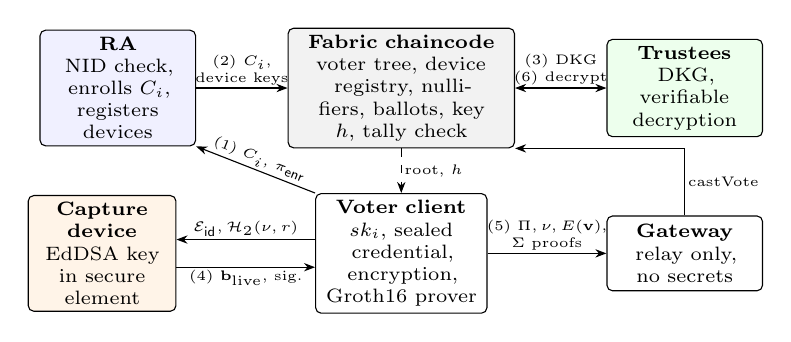
\begin{tikzpicture}[font=\scriptsize, >={Stealth[length=4pt]},
            box/.style={draw, rounded corners=2pt, align=center, inner sep=2.5pt, minimum height=0.95cm},
            lbl/.style={font=\tiny, align=center, inner sep=1pt}]
          \node[box, fill=blue!6,   text width=1.8cm] (RA) at (0,2.1)   {\textbf{RA}\\NID check, enrolls $C_i$, registers devices};
          \node[box, fill=gray!10,  text width=2.7cm] (L)  at (3.6,2.1) {\textbf{Fabric chaincode}\\voter tree, device registry, nullifiers, ballots, key $h$, tally check};
          \node[box, fill=green!7,  text width=1.8cm] (TA) at (7.2,2.1) {\textbf{Trustees}\\DKG, verifiable decryption};
          \node[box, fill=orange!9, text width=1.7cm] (D)  at (-0.2,0)  {\textbf{Capture device}\\EdDSA key in secure element};
          \node[box,                text width=2.0cm] (V)  at (3.6,0)   {\textbf{Voter client}\\$sk_i$, sealed credential, encryption, Groth16 prover};
          \node[box,                text width=1.8cm] (G)  at (7.2,0)   {\textbf{Gateway}\\relay only, no secrets};
          \draw[->] (V.north west) -- node[lbl, sloped, above] {(1) $C_i$, $\pi_{\mathsf{enr}}$} (RA.south east);
          \draw[->] (RA.east) -- node[lbl, above] {(2) $C_i$,\\device keys} (L.west);
          \draw[<->] (TA.west) -- node[lbl, above] {(3) DKG\\(6) decrypt} (L.east);
          \draw[->] ([yshift=5pt]V.west) -- node[lbl, above] {$\mathcal{E}_{\mathsf{id}}, \mathcal{H}_2(\nu,r)$} ([yshift=5pt]D.east);
          \draw[->] ([yshift=-5pt]D.east) -- node[lbl, below] {(4) $\mathbf{b}_{\text{live}}$, sig.} ([yshift=-5pt]V.west);
          \draw[->] (V.east) -- node[lbl, above] {(5) $\Pi, \nu, E(\mathbf{v})$,\\$\Sigma$ proofs} (G.west);
          \draw[->] (G.north) -- node[lbl, right] {castVote} (G.north |- L.south east) -- (L.south east);
          \draw[->, dashed] (L.south) -- node[lbl, right] {root, $h$} (V.north);
        \end{tikzpicture}}
        \caption{System architecture. (1)--(2)~attested enrollment: a kiosk signs the template for the NID and the client proves $C_i$ opens to it; (3)~trustee DKG through the chaincode; (4)~attested capture bound to the election and a hidden nullifier; (5)~the client-built ballot, relayed and fully checked on-chain; (6)~verified threshold decryption of the totals.}
        \label{fig:architecture}
    \end{minipage}\hfill
    \begin{minipage}{0.48\textwidth}
        \centering
        \resizebox{\linewidth}{!}{%
        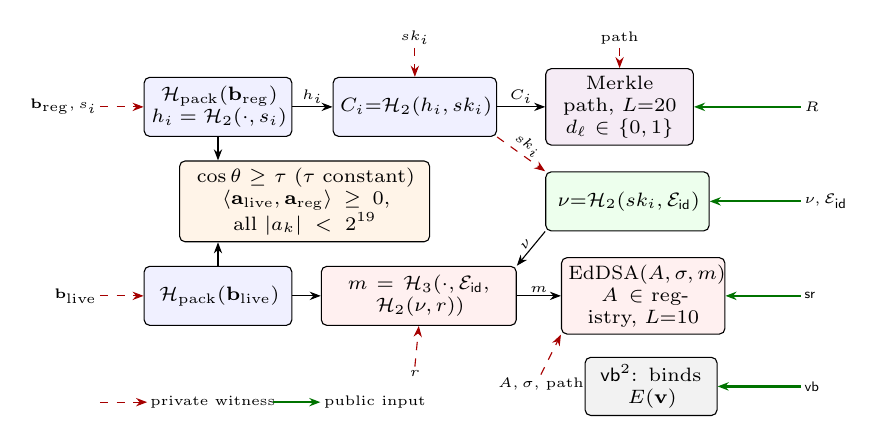
\begin{tikzpicture}[font=\scriptsize, >={Stealth[length=4pt]},
            blk/.style={draw, rounded corners=2pt, align=center, inner sep=2.5pt, minimum height=0.75cm},
            priv/.style={->, draw=red!65!black, dashed},
            pub/.style={<-, draw=green!45!black, thick},
            lbl/.style={font=\tiny, align=center, inner sep=1pt}]
          % row 1: enrolled template -> commitment -> membership
          \node[blk, fill=blue!6,   text width=1.7cm] (HR) at (0.9,3.0) {$\mathcal{H}_{\text{pack}}(\mathbf{b}_{\text{reg}})$\\$h_i = \mathcal{H}_2(\cdot, s_i)$};
          \node[blk, fill=blue!6,   text width=1.9cm] (CM) at (3.4,3.0) {$C_i{=}\mathcal{H}_2(h_i, sk_i)$};
          \node[blk, fill=violet!8, text width=1.7cm] (MK) at (6.0,3.0) {Merkle path, $L{=}20$\\$d_\ell \in \{0,1\}$};
          % row 2: comparator and nullifier
          \node[blk, fill=orange!9, text width=3.0cm] (CS) at (2.0,1.8) {$\cos\theta \ge \tau$ ($\tau$ constant)\\$\langle \mathbf{a}_{\text{live}}, \mathbf{a}_{\text{reg}} \rangle \ge 0$, all $|a_k| < 2^{\nCoordBits}$};
          \node[blk, fill=green!7,  text width=1.9cm] (NL) at (6.1,1.8) {$\nu{=}\mathcal{H}_2(sk_i, \mathcal{E}_{\mathsf{id}})$};
          % row 3: attestation
          \node[blk, fill=blue!6,   text width=1.7cm] (HL) at (0.9,0.6) {$\mathcal{H}_{\text{pack}}(\mathbf{b}_{\text{live}})$};
          \node[blk, fill=red!6,    text width=2.3cm] (MS) at (3.45,0.6) {$m = \mathcal{H}_3(\cdot, \mathcal{E}_{\mathsf{id}},$\\$\mathcal{H}_2(\nu, r))$};
          \node[blk, fill=red!6,    text width=1.9cm] (ED) at (6.3,0.6) {EdDSA$(A, \sigma, m)$\\$A \in$ registry, $L{=}10$};
          % row 4: ballot binding
          \node[blk, fill=gray!10,  text width=1.5cm, minimum height=0.55cm] (VB) at (6.4,-0.55) {$\mathsf{vb}^2$: binds $E(\mathbf{v})$};
          % internal flow
          \draw[->] (HR) -- node[lbl, above] {$h_i$} (CM);
          \draw[->] (CM) -- node[lbl, above] {$C_i$} (MK);
          \draw[->] (HR.south) -- (HR.south |- CS.north);
          \draw[->] (HL.north) -- (HL.north |- CS.south);
          \draw[->] (HL) -- (MS);
          \draw[->] (MS) -- node[lbl, above] {$m$} (ED);
          \draw[->] (NL.south west) -- node[lbl, above, sloped] {$\nu$} (MS.north east);
          % private witnesses
          \draw[priv] (-0.6,3.0) node[left, lbl] {$\mathbf{b}_{\text{reg}}, s_i$} -- (HR.west);
          \draw[priv] (-0.6,0.6) node[left, lbl] {$\mathbf{b}_{\text{live}}$} -- (HL.west);
          \draw[priv] (3.4,3.75) node[above, lbl] {$sk_i$} -- (CM.north);
          \draw[priv] (CM.south east) -- node[lbl, above, sloped] {$sk_i$} (NL.north west);
          \draw[priv] (6.0,3.75) node[above, lbl] {path} -- (MK.north);
          \draw[priv] (3.4,-0.3) node[below, lbl] {$r$} -- (MS.south);
          \draw[priv] (5.0,-0.4) node[below, lbl] {$A, \sigma$, path} -- (ED.south west);
          % public inputs
          \draw[pub] (MK.east) -- (8.3,3.0) node[right, lbl] {$R$};
          \draw[pub] (NL.east) -- (8.3,1.8) node[right, lbl] {$\nu, \mathcal{E}_{\mathsf{id}}$};
          \draw[pub] (ED.east) -- (8.3,0.6) node[right, lbl] {$\mathsf{sr}$};
          \draw[pub] (VB.east) -- (8.3,-0.55) node[right, lbl] {$\mathsf{vb}$};
          % legend
          \draw[priv] (-0.6,-0.75) -- (0.0,-0.75) node[right, lbl] {private witness};
          \draw[->, draw=green!45!black, thick] (1.6,-0.75) -- (2.2,-0.75) node[right, lbl] {public input};
        \end{tikzpicture}}
        \caption{The face eligibility circuit. Private witnesses (dashed) never leave the client; the public inputs are the voter-tree root $R$, the nullifier $\nu$, the election identifier $\mathcal{E}_{\mathsf{id}}$, the device-registry root $\mathsf{sr}$ and the ballot binding $\mathsf{vb}$. The threshold is a circuit constant.}
        \label{fig:zkp_circuit}
    \end{minipage}
\end{figure*}


\subsection{System Entities}
The architecture (Fig.~\ref{fig:architecture}) defines five interacting entity classes:

\paragraph{Voters ($\mathcal{V}$)} Each voter $\mathcal{V}_i$ enrolls to cast one ballot in election $\mathcal{E}$, presenting a national ID (NID), password $\text{pwd}_i$, and a biometric reading; the voter's client generates the private key $sk_i \in \mathbb{F}_p$ ($sk_i \neq 0$), salt $s_i$ and template, and keeps them in a credential file encrypted under $\text{pwd}_i$. To vote, the voter presents their face at a capture kiosk and builds, proves and submits the ballot on their own client device. Voters keep physical custody of their biometric traits under Assumption~\ref{asm:uncloneable}.

\paragraph{Registration Authority ($\mathcal{RA}$)} Validates NIDs against civil registries, supervises enrollment capture, and publishes the client's commitment $C_i = \mathcal{H}_2(h_i, sk_i)$ to tree $\mathcal{T}$ without seeing $sk_i$, $s_i$ or the template. The RA cannot see whether $C_i$ encodes the enrollee's face, so enrollment is attested: a registered kiosk signs the template it captured for the NID the RA verified, and the client proves that $C_i$ opens to it (\S\ref{sec:protocol_construction}-B). It registers capture devices, opens and closes ballots, but cannot decrypt ballots or forge proofs. The RA is trusted for eligibility: a corrupt RA can enroll phantom leaves or register a rogue device, and the ledger records each action append-only but cannot check it against the civil registry. The prototype indexes enrollments by $\mathsf{SHA256}(\text{NID})$, which anyone can enumerate over the low-entropy NID space to learn who enrolled; a deployment should use $\mathsf{HMAC}$ under an RA key instead.

\paragraph{Capture Kiosks ($\mathcal{D}$)} Supervised camera terminals at polling stations, each holding an EdDSA key in a secure element that the RA registers on-chain (registry of $2^{10}$ kiosks). A kiosk captures the face, extracts the template and signs it for one election and one hidden nullifier; it never sees the voter's credential, nullifier or vote. For eligibility we assume kiosk keys cannot be extracted. Unsupervised remote voting, where the camera is the voter's own phone, is out of scope: it would need hardware-backed keys with platform key attestation and a much larger registry.

\paragraph{Trustees ($\mathcal{TA}_1, \ldots, \mathcal{TA}_n$)} Jointly generate the election key so that no party knows it, and after closure decrypt only the homomorphic totals; any $t$ of them suffice and any $t-1$ learn nothing.

\paragraph{Permissioned Ledger ($\mathcal{L}$)} On Hyperledger Fabric, maintains append-only total ordering, enforces MVCC state updates, and hosts voting smart contracts; privacy rests entirely on cryptographic blinding and zero-knowledge arguments.


\subsection{Threat Model and Trust Assumptions}
We consider a PPT adversary $\mathcal{A}$ who may corrupt a subset of system entities across five classes ($\mathcal{A}_{\mathcal{V}}, \mathcal{A}_{\mathcal{RA}}, \mathcal{A}_{\mathcal{D}}, \mathcal{A}_{\mathcal{TA}}, \mathcal{A}_{\mathcal{L}}$), summarized in Table~\ref{tab:threat_matrix}. Following standard e-voting models (Helios~\cite{Adida2008}, Semaphore~\cite{Gurkan2020}), we protect eligibility, anonymity, integrity, and anti-replay against active network/infrastructure adversaries; receipt-freeness and coercion resistance are out of scope (\S\ref{sec:limitations}).

\begin{table}[t]
\caption{Threat Matrix and Mitigations}
\label{tab:threat_matrix}
\centering
\footnotesize
\setlength{\tabcolsep}{2.5pt}
\renewcommand{\arraystretch}{0.90}
\resizebox{\columnwidth}{!}{%
\begin{tabular}{@{}llp{4.3cm}@{}}
\toprule
\textbf{Adversary} & \textbf{Attack Vector} & \textbf{Mitigation} \\
\midrule
$\mathcal{A}_{\mathcal{V}}$ (Voter) 
  & Double voting & Deterministic nullifier $\nu$; chaincode rejects a reused $\nu$. \\
  & Impersonation & zk-SNARK enforces biometric similarity $\leq \delta$. \\
  & Ballot stuffing & Disjunctive Chaum--Pedersen ($v_j \in \{0,1\}$). \\
  & Credential share & Live sample must carry an in-circuit-verified signature of a registered capture device. \\
  & Enroll another's face & Kiosk-attested enrollment proof bound to the NID (A25--A27). \\
\midrule
$\mathcal{A}_{\mathcal{RA}}$ (RA)
  & Phantom voter, rogue kiosk & Not prevented (RA trusted for eligibility); enrollments and kiosk keys are append-only and auditable. \\
  & Who enrolled & Prototype: enumerable $\mathsf{SHA256}(\text{NID})$; deployment: HMAC under an RA key. \\
  & Template theft & RA sees only the Poseidon commitment $C_i$. \\
  & Key theft & $sk_i$ generated and sealed client-side. \\
\midrule
$\mathcal{A}_{\mathcal{D}}$ (Kiosk)
  & Ballot linkage & Signs $\mathcal{H}_2(\nu, r)$, never $\nu$; capture timing is residual (\S\ref{sec:anonymity}). \\
\midrule
$\mathcal{A}_{\mathcal{TA}}$ (Trustee)
  & Early decrypt & $t$-of-$n$ DKG key; closed ballot required for any tally. \\
  & Tally forgery & Chaincode checks $t$ partial-decryption proofs per total. \\
  & Voter exclusion & Append-only ledger; public audit log. \\
\bottomrule
\end{tabular}%
}
\end{table}

\subsection{Security Definitions}

\begin{assumption}[Biometric Unforgeability modulo Matching Tolerance ($\delta$)]
\label{asm:uncloneable}
For an honest registered voter $\mathcal{V}_i$ with enrolled biometric template $\mathbf{b}_i$, no PPT adversary $\mathcal{A}$ without physical coercion can synthesize or present a biometric feature vector $\mathbf{b}'$ such that $\mathrm{dist}(\mathbf{b}', \mathbf{b}_i) \leq \delta$, except with probability bounded by the False Acceptance Rate $\mathsf{FAR}_\delta$. A live sample counts only if a registered capture device signed it, which the circuit verifies (\S\ref{sec:protocol_construction}-C); we assume the device performs presentation attack detection (PAD) before signing, outside the proof; the prototype attestor does not, and we do not evaluate PAD (\S\ref{sec:limitations}).
\end{assumption}

We formalize five electoral security goals, proved in Section~\ref{sec:security}:
\begin{enumerate}[leftmargin=*,noitemsep,topsep=1pt,parsep=0pt]
    \item \textbf{Eligibility Soundness:} A ballot is accepted only for an enrolled credential backed by a genuine attested presentation, except with probability $q \cdot \mathsf{FAR}_\delta + \mathsf{negl}(\lambda)$ after $q$ impostor presentations (Theorem~\ref{thm:eligibility}).
    \item \textbf{One Vote per Credential:} At most one ballot per credential and election is accepted (Theorem~\ref{thm:antireplay}).
    \item \textbf{Ballot Integrity:} Accepted ballots encrypt a unit vector and cannot be substituted, copied or front-run (Theorem~\ref{thm:integrity}).
    \item \textbf{Ballot Privacy and Unlinkability:} Ballots reveal neither the choice nor the voter, even to the RA, gateway, capture devices and any $t-1$ trustees (Theorem~\ref{thm:anonymity}).
    \item \textbf{Universal Verifiability:} Any auditor can verify every ballot and the correct decryption of every total from public data (Proposition~\ref{prop:verif}).
\end{enumerate}


\subsection{Cryptographic Preliminaries}

\subsubsection{Poseidon Hash Function}
Poseidon~\cite{Grassi2021} is an algebraic hash family over $\mathbb{F}_p$ ($p \approx 2.189 \times 10^{76}$) optimized for SNARKs. We use $\text{Poseidon}_{11}$ over packed coordinates for template hashing and $\text{Poseidon}_2$ for 2-to-1 Merkle updates and nullifiers. An arity-2 Poseidon instance costs 240 R1CS constraints here, two orders of magnitude fewer than SHA-256.

\begin{assumption}[Poseidon Hash Security]
\label{asm:poseidon}
Poseidon over $\mathbb{F}_p$~\cite{Grassi2021} satisfies collision resistance ($\mathbf{Adv}^{\mathsf{CR}}_{\mathsf{Pos}}(\lambda) \in \mathsf{negl}(\lambda)$), and preimage resistance ($\mathbf{Adv}^{\mathsf{Pre}}_{\mathsf{Pos}}(\lambda) \in \mathsf{negl}(\lambda)$); where hiding is needed we model it as a random oracle.
\end{assumption}

\subsubsection{Groth16 zk-SNARK}
Groth16~\cite{Groth2016} provides minimal proof size and rapid verification over pairing-friendly curve BN254 ($E: y^2 = x^3 + 3 \bmod q$). Proof $\Pi = (\pi_A \in \mathbb{G}_1, \pi_B \in \mathbb{G}_2, \pi_C \in \mathbb{G}_1)$ spans 128 bytes compressed; it is knowledge-sound in the algebraic group model~\cite{Fuchsbauer2018} and weakly simulation-extractable~\cite{Baghery2021}.

\subsubsection{Exponential ElGamal Encryption}
Exponential ElGamal over secp256k1 (generator $G$, order $n$) provides additive homomorphism for tallying. For public key $h = xG$ and bit $m \in \{0, 1\}$, $E(m; r) = (rG, mG + rh)$ with randomness $r \xleftarrow{\$} \mathbb{Z}_n^*$. Additive homomorphism allows tally aggregation without individual decryption: $\bigoplus_{i=1}^{N} E(m_i; r_i) = ((\sum_i r_i)G, (\sum_i m_i)G + (\sum_i r_i)h)$, secure under DDH.

\subsubsection{Disjunctive Chaum--Pedersen Proof}
Voters attach a non-interactive zero-knowledge disjunctive Chaum--Pedersen proof ($\Sigma$-OR)~\cite{ChaumPedersen1992} to each ciphertext component $E(v_j)$, proving $v_j \in \{0, 1\}$ without disclosing $v_j$ under discrete-logarithm hardness.

\subsubsection{Voter Merkle Tree}
Voter eligibility commitments populate an append-only binary Merkle tree of fixed depth $L = 20$ ($2^{20} \approx 1.04 \times 10^6$ leaf capacity). Membership is proven in-circuit with $\text{Poseidon}_2$; a forged opening yields a Poseidon collision (Lemma~\ref{lem:merkle-binding}).

\subsubsection{Circuit-Optimized Biometric Matching Metrics}
\label{sec:metric_formulation}
Circuit cost grows with the output dimension $d$ of the encoding $\phi: \mathcal{X} \to \mathcal{Y}$, so we select $(d, \tau)$ by a rule fixed before any test data is used: on validation identities, $\tau_d$ is the lowest threshold at which a lookalike attacker screening $K = 100$ candidates succeeds against at most 1\% of targets, and we deploy the smallest $d$ whose FRR at $\tau_d$ is at most 1\%, the cheapest circuit that meets both error targets. Neither ITQ~\cite{Gong2013} (accuracy alone) nor naive truncation (constraint count alone) targets this, and we evaluate the whole sweep rather than a single point (\S\ref{subsec:eval_encoding}).
The deployed encoding is PCA of a 512-D ArcFace embedding~\cite{Deng2019ArcFace}, fitted on the training identities, $\hat{\mathbf{v}} = \mathbf{W}(\mathbf{v} - \boldsymbol{\mu}) / \|\mathbf{W}(\mathbf{v} - \boldsymbol{\mu})\|_2$ with $\mathbf{W} \in \mathbb{R}^{128 \times 512}$, $\mathbf{W}\mathbf{W}^T = \mathbf{I}_{128}$. We also evaluate Spherical Orthogonal Projection and Quantization (SOPQ), which learns $\mathbf{W}$ from a shrinkage-regularized Fisher discriminant (between- vs.\ within-identity scatter) and orthonormalizes it by QR, on the hypothesis that a discriminant projection should beat reconstruction-optimal PCA; it does only at $d \le 32$ (\S\ref{subsec:eval_encoding}). Fixed-point scaling with $\sigma = \nSigma$ gives integers $a_k = \lfloor \sigma \hat{v}_k \rceil$, $|a_k| \le \sigma < 2^{\nCoordBits}$. Inside the circuit, $\cos\theta \ge \tau$ is evaluated without division or square roots:
\begin{equation}
\label{eq:sopq-circuit}
\langle \mathbf{a}_{\text{live}}, \mathbf{a}_{\text{reg}} \rangle^2 \cdot \tau_{\mathsf{den}} \;\ge\; \tau_{\mathsf{num}} \cdot \|\mathbf{a}_{\text{live}}\|^2 \cdot \|\mathbf{a}_{\text{reg}}\|^2
\end{equation}
with $\tau_{\mathsf{num}} = 1225$ and $\tau_{\mathsf{den}} = 10^4$ ($\tau = 0.35$) fixed in the circuit, plus $\langle \mathbf{a}_{\text{live}}, \mathbf{a}_{\text{reg}} \rangle \ge 0$. Because the prover chooses the witness, an honest quantizer does not bound the values; the circuit range-checks every coordinate to $|a_k| < 2^{\nCoordBits}$, which keeps both sides below $2^{\nCmpBits} \ll p \approx 2.19 \times 10^{76}$ (BN254), so the field inequality equals the integer one.

\subsubsection{Key Derivation}
PBKDF2 with HMAC-SHA-256 (600,000 iterations) derives a 256-bit AES key from the voter's password $\text{pwd}_i$ for local credential storage (AES-256-GCM).


% --- Section 4 : Protocol Construction ---%

\section{Protocol Construction}
\label{sec:protocol_construction}

This section presents the protocol in five phases: key generation, registration, authentication, vote casting, and tallying.

\subsection{Key Generation and Commitment Scheme}

\subsubsection{Voter Credential Generation}
During registration, each voter's client samples a secret key $sk_i \leftarrow \{0,1\}^{256} \bmod 2^{252}$ ($sk_i \neq 0$) in $\mathbb{F}_p$, avoiding modular wrap-around in BN254 circuits. Given biometric template $\mathbf{b}_i$ and random salt $s_i \xleftarrow{\$} \mathbb{F}_p$, the client computes biometric hash $h_i = \mathcal{H}_{\text{pack}}(\mathbf{b}_i, s_i)$ and on-chain commitment leaf:
\begin{equation}
\label{eq:commitment-leaf}
C_i = \mathcal{H}_2(h_i, sk_i) = \mathcal{H}_2(\mathcal{H}_{\text{pack}}(\mathbf{b}_i, s_i), sk_i)
\end{equation}
where $\mathcal{H}_{\text{pack}}$ offsets each coordinate of $\mathbf{b}_i \in \mathbb{Z}^{128}$ by $2^{\nCoordBits}$ into a \nRangePerCoord-bit slot, packs 12 slots per field element (11 elements) and applies one Poseidon, salted via $h_i = \mathcal{H}_2(h_{\text{emb}}, s_i)$. This cryptographically binds $\mathbf{b}_i$ to the enrollment salt $s_i$ and $h_i$ to secret key $sk_i$.

\subsubsection{Threshold Election Key}
The registrar registers the ballot with $n$ trustee signing keys and a threshold $t$. The trustees run Pedersen's joint-Feldman DKG~\cite{Pedersen1991,Feldman1987} through the chaincode. Trustee $k$ posts signed commitments $A_{k\ell} = a_{k\ell} G$ to a random degree-$(t-1)$ polynomial $f_k$ and sends $f_k(m)$ privately to each trustee $m$. A share inconsistent with the commitments is revealed in a signed complaint, and the chaincode disqualifies its dealer. The chaincode then \emph{derives} $h = \sum_{k \in \mathsf{QUAL}} A_{k0}$ ($|\mathsf{QUAL}| \ge t$) and opens voting. Trustee $m$ holds $x_m = \sum_k f_k(m)$, and its verification key $h_m = x_m G$ is publicly computable from the commitments.

\subsection{Voter Registration Phase}
Registration is a one-time supervised operation in five steps:
(i)~\textbf{Identity Deduplication:} $\text{nidHash} = \mathsf{SHA256}(\text{NID})$ (keyed in deployment, \S\ref{sec:system_model}) is checked against on-chain records;
(ii)~\textbf{Biometric Extraction:} an SCRFD detector~\cite{Guo2022SCRFD} with five-point alignment and an ArcFace ResNet-50 trained on WebFace600K~\cite{Zhu2021WebFace260M} (InsightFace \texttt{buffalo\_l}) yield 512-D embeddings, projected via PCA to 128 dimensions and scaled by $\sigma = \nSigma$;
(iii)~\textbf{Attested Commitment:} the kiosk signs $\mathcal{H}_3(\mathcal{H}_{\text{pack}}(\mathbf{b}_i), D_{\mathsf{enr}}, \mathcal{H}_2(n_i, 0))$ for the NID the RA entered, $n_i = \mathrm{trunc}_{248}\mathsf{SHA256}(\text{nidHash})$, where $D_{\mathsf{enr}} = 2^{200}$ exceeds every $\mathcal{E}_{\mathsf{id}}$ so enrollment and vote signatures cannot be swapped; the client computes $C_i = \mathcal{H}_2(h_i, sk_i)$ and a Groth16 proof $\pi_{\mathsf{enr}}$ (\nEnrollConstraints{} constraints, \nBrowserEnrollMs~ms in a browser) that $C_i$ opens to the signed template, range checks included;
(iv)~\textbf{On-Chain Enrollment:} the RA submits $(\text{nidHash}, C_i, \pi_{\mathsf{enr}})$; the chaincode checks $\pi_{\mathsf{enr}}$ against $C_i$, $n_i$ and the device-registry root, and $C_i$ is appended to tree $\mathcal{T}$;
(v)~\textbf{Credential Storage:} Credentials are encrypted client-side via AES-256-GCM and PBKDF2 under password $\text{pwd}_i$.

\subsection{Authentication and zk-SNARK Proof Generation}
Authentication produces a Groth16 proof $\Pi$ attesting to biometric similarity, commitment, Merkle membership, and nullifiers without revealing witnesses. The Circom~\cite{Circom2023} circuit (\texttt{face\_auth.circom}, compiler 2.2.3 with \texttt{--O2}) has $\nFaceConstraints$ R1CS constraints, with public signals $(R, \nu, \mathcal{E}_{\mathsf{id}}, \mathsf{vb}, \mathsf{sr})$. It comprises five sub-circuits (Fig.~\ref{fig:zkp_circuit}), each measured in isolation (Supplementary Material, Table~S2):
(i)~\textbf{Template hashing:} $\mathcal{H}_{\text{pack}}$ over the enrolled and the live sample ($2 \times \nHashConstraints$; per-coordinate Poseidon chunks would cost $2 \times \nChunkedHash$). Packing is a linear map and adds no constraints, but it is injective only because (iii) range-checks every coordinate: without that, carries between slots let a stolen credential open its commitment with a template steered towards the attacker's face (attack A24).
(ii)~\textbf{MerkleTreeChecker:} computes $c_{\ell+1} = \mathsf{Poseidon}_2(\mathsf{Switcher}(c_\ell, p_\ell, d_\ell))$ across $L=20$ levels with each $d_\ell$ constrained to $\{0,1\}$, asserting $c_{20} = \mathcal{R}$ ($\nMerkleConstraints$).
(iii)~\textbf{Distance Comparator:} Eq.~\eqref{eq:sopq-circuit} with $\tau$ fixed in the circuit, every coordinate range-checked to $|a_k| < 2^{\nCoordBits}$ and $\langle \mathbf{a}_{\text{live}}, \mathbf{a}_{\text{reg}} \rangle \geq 0$ enforced ($\nCosConstraints$, of which $\nRangeConstraints$ are range checks). With packing, these range checks are the main cost that grows with $d$; membership and attestation are fixed.
(iv)~\textbf{Salt, Commitment and Nullifier:} three $\text{Poseidon}_2$ evaluations, including $\nu = \text{Poseidon}_2(sk_i, \mathcal{E}_{\mathsf{id}})$ ($3 \times \nPoseidonTwo$).
(v)~\textbf{Sensor Attestation} ($\nAttestConstraints$): Without it, the live sample is a free witness and the proof shows only knowledge of the template. The circuit verifies an EdDSA-Poseidon signature over $\text{Poseidon}_3(\mathcal{H}_{\text{pack}}(\mathbf{b}_{\text{live}}), \mathcal{E}_{\mathsf{id}}, \text{Poseidon}_2(\nu, r))$ by a key lying in a depth-10 device registry whose root is public. The hiding commitment $\text{Poseidon}_2(\nu, r)$ makes each signature valid for one vote while preventing the device from linking the capture to the ballot.
The voter client computes the witness and the Groth16 proof with snarkjs's WASM prover (\nClientS~s per ballot in total, Table~\ref{tab:combined_metrics}); signal tables are in Supplementary Material, Appendix~B.

\subsection{Vote Casting}
Ballot $\mathcal{B}$'s election identifier is $\mathcal{E}_{\mathsf{id}} = \text{trunc}_{128}(\mathsf{SHA256}(\mathcal{B}.\text{id}))$.
The client encrypts the one-hot vector $\mathbf{v} \in \{0,1\}^k$ under $h$, $E(v_j) = (r_j G, v_j G + r_j h)$, attaches $\Sigma$-OR proofs $\pi_j^{\mathsf{val}}$~\cite{ChaumPedersen1992} that $v_j \in \{0,1\}$ and a Chaum--Pedersen proof that $\sum_j v_j = 1$, with strong Fiat--Shamir challenges $e = \mathsf{SHA256}(h \parallel c_{1,j} \parallel c_{2,j} \parallel a_1 \parallel b_1 \parallel a_2 \parallel b_2 \parallel \mathcal{B}.\text{id} \parallel \nu \parallel j) \bmod n$, and proves $\Pi$ with $\mathsf{vb}$ binding $E(\mathbf{v})$. In one transaction the chaincode checks that the ballot is open, then $\Pi$, the root, $\mathcal{E}_{\mathsf{id}}$, the sensor root, $\mathsf{vb}$, every ballot proof, and that $\nu$ is unused, then appends $(\nu, E(\mathbf{v}), \boldsymbol{\pi})$.

\subsection{Homomorphic Tallying and Result Decryption}
\textbf{Step 1: Ciphertext Aggregation.} Tallying accumulates ciphertexts via additive homomorphism:
\begin{equation}
  \hat{E}(T_j) = \sum_{i=1}^{N} E(v_{i,j}) = \left( \sum_{i=1}^{N} r_{i,j} G, \; T_j G + \sum_{i=1}^{N} r_{i,j} h \right)
\end{equation}
\textbf{Step 2: Threshold Decryption.} After the registrar closes the ballot on-chain, $t$ trustees each publish $D_{k,j} = x_k \hat{c}_{1,j}$ with a DLEQ proof $\pi_{k,j}^{\mathsf{dec}}$ that $\log_G h_k = \log_{\hat{c}_{1,j}} D_{k,j}$, where $h_k$ is computable from the on-chain commitments. Lagrange interpolation gives $M_j = \hat{c}_{2,j} - \sum_k \lambda_k D_{k,j} = T_j G$, solved for $T_j$ by Baby-Step Giant-Step in $\mathcal{O}(\sqrt{N})$. \texttt{publishTally} recomputes every aggregate from the stored ballots and accepts the totals only with at least $t$ valid partial decryptions per option that open it to exactly $T_j$ (write-once).

\section{Security Analysis}
\label{sec:security}

We state security as game-based properties over the public ledger. We deliberately do not claim UC security: Groth16 is knowledge-sound only via non-black-box extraction in the algebraic group model, and its proofs are re-randomizable, so it lacks the straight-line, simulation-extractable proofs a UC simulator needs~\cite{Baghery2021}. Each property below is tied to a constraint or chaincode check of the implementation and is exercised by the attack suite of Section~\ref{sec:implementation_and_evaluation}; full proofs are in Supplementary Material, Appendix~C.

\subsection{Adversary and Assumptions}
\label{sec:assumptions}
The PPT adversary $\mathcal{A}$ controls the network and the API gateway, statically corrupts any set of voters, may steal credential files, and observes the whole ledger. For privacy it additionally controls the RA after enrollment and every capture device; for eligibility, capture devices are honest. For privacy at most $t-1$ trustees are corrupt, and the election key is unbiased. A corrupt trustee can bias the key of Pedersen's joint-Feldman DKG, which we implement. Gennaro et al.\ show the bias harmless for schemes whose security reduces to discrete logarithms~\cite{Gennaro2003}, but ElGamal's privacy rests on DDH, so we keep the assumption; their bias-free variant~\cite{Gennaro2007} adds one commitment round, which the chaincode can host unchanged. We assume:
(A1)~Groth16 is perfectly zero-knowledge and knowledge-sound in the AGM~\cite{Groth2016,Fuchsbauer2018}, and weakly simulation-extractable: given simulated proofs, $\mathcal{A}$ cannot prove a statement outside that set~\cite{Baghery2021};
(A2)~Assumption~\ref{asm:poseidon}, with Poseidon modeled as a random oracle where hiding is needed;
(A3)~DDH in secp256k1, and the $\Sigma$-OR, sum-to-one and decryption proofs are Fiat--Shamir transforms of special-sound HVZK $\Sigma$-protocols that hash the full statement and a context (strong Fiat--Shamir), hence sound and zero-knowledge in the ROM~\cite{fiat1987how,Bernhard2012};
(A4)~EdDSA over BabyJubJub with Poseidon as its hash is EUF-CMA, modeling Poseidon as a random oracle~\cite{Bernstein2012}; circomlib's verifier rejects $S$ outside the prime-order subgroup's range and small-order keys ($8A \neq \mathcal{O}$) and checks the cofactor-cleared equation;
(A5)~Assumption~\ref{asm:uncloneable} holds per presentation, with false-accept rate $\mathsf{FAR}_\delta$.

\begin{assumption}[Fabric Consensus Safety]
\label{asm:fabric}
Under Fabric's execute-order-validate architecture with Raft consensus, committed transactions are totally ordered and validated against world state at commit time (MVCC read-before-write).
\end{assumption}

\subsection{Eligibility and One Vote per Credential}
\label{sec:eligibility}

\begin{lemma}[Merkle Binding]
\label{lem:merkle-binding}
If every direction bit $d_\ell$ is constrained to $\{0,1\}$, any opening $(C^\ast, \{(\sigma_\ell, d_\ell)\}_{\ell<L})$ of root $R$ with $C^\ast \notin \{C_1,\ldots,C_m\}$ yields a Poseidon collision, so $\Pr[\text{forgery}] \leq \mathbf{Adv}^{\mathsf{CR}}_{\mathsf{Pos}}(\lambda)$.
\end{lemma}

\begin{proof}[Proof Sketch]
Walk the forged and canonical paths from the root; the first level at which the hashed pairs differ is a collision. The booleanity constraint is essential: circomlib's \texttt{Switcher} does not enforce it, and with a free $d_{L-1}$ the prover can solve $L + d(R'-L) = x$, $R' - d(R'-L) = y$ for the root's children $(x,y)$ from \emph{any} leaf (attack A1 in Table~\ref{tab:attack_suite}).
\end{proof}

\begin{theorem}[Eligibility Soundness]
\label{thm:eligibility}
Let $\mathcal{A}$ make at most $q$ presentations to registered capture devices that are not genuine presentations of the enrolled voter whose credential it uses. The probability that the ledger accepts a ballot whose credential is neither corrupt nor backed by a genuine presentation is at most
\begin{equation}
\label{eq:eligibility-bound}
\varepsilon^{\mathsf{ks}}_{\mathsf{G16}}(\lambda) + 4\,\mathbf{Adv}^{\mathsf{CR}}_{\mathsf{Pos}}(\lambda) + \mathbf{Adv}^{\mathsf{EUF}}_{\mathsf{EdDSA}}(\lambda) + q \cdot \mathsf{FAR}_\delta .
\end{equation}
\end{theorem}

\begin{proof}[Proof Sketch]
Extract a witness from the accepted proof (A1). Poseidon collision resistance is used four times, once per binding below. (i)~By Lemma~\ref{lem:merkle-binding}, $C$ is an enrolled leaf, and (ii)~$C = \mathcal{H}_2(\mathcal{H}_{\text{pack}}(\mathbf{b}_{\text{reg}}, s), sk)$ opens to the enrolled template, since packing is injective on range-checked coordinates (step (v); attack A24). (iii)~The device key opens the registry root that the chaincode checks (Lemma~\ref{lem:merkle-binding} again), so it is registered; unless EdDSA is forged, that device signed $m = \mathcal{H}_3(\mathcal{H}_{\text{pack}}(\mathbf{b}_{\text{live}}), \mathcal{E}_{\mathsf{id}}, \mathcal{H}_2(\nu, r))$, and (iv)~$m$ determines $\mathbf{b}_{\text{live}}$, i.e., the device captured $\mathbf{b}_{\text{live}}$ for this election and this nullifier (attacks A6, A13--A16). (v)~The threshold is a circuit constant fixed by the verification key, every coordinate is range-checked to $|a_k| < 2^{\nCoordBits}$ so no product wraps modulo $p$, and $\langle \mathbf{a}_{\text{live}}, \mathbf{a}_{\text{reg}}\rangle \geq 0$ is enforced, since squaring otherwise accepts $\cos\theta \le -\tau$ (attacks A2, A5). Hence $\mathrm{dist}(\mathbf{b}_{\text{live}}, \mathbf{b}_{\text{reg}}) \le \delta$, which a non-genuine presentation achieves with probability $\mathsf{FAR}_\delta$; a union bound over $q$ presentations completes the proof.
\end{proof}

\textbf{Instantiating $\mathsf{FAR}_\delta$: the Biometric as a Second Factor.} A presentation helps $\mathcal{A}$ only after it holds the victim's credential file and password, so the biometric bounds an attacker who has stolen the first factor. A face is public, so that attacker screens candidates' photos offline and recruits the best match; rate-limiting does not stop a \emph{single} presentation.

\begin{definition}[$K$-Screening Impersonation]
\label{def:lookalike}
The challenger samples a target identity $t$ and $K$ candidate identities, independently of $t$, and gives $\mathcal{A}$ public photos of all of them. $\mathcal{A}$ recruits one candidate, who presents once at a registered kiosk; $\mathcal{A}$ wins if the circuit accepts against $t$'s template. $\mathsf{Adv}^{\mathsf{look}}_K(\tau)$ is its winning probability.
\end{definition}

\begin{proposition}
\label{prop:lookalike}
$\mathsf{Adv}^{\mathsf{look}}_K(\tau) \le 1 - (1 - \mathsf{FAR})^K \le K \cdot \mathsf{FAR}$, with $\mathsf{FAR}$ the zero-effort rate at $\tau$, so Theorem~\ref{thm:eligibility} holds with $\mathsf{FAR}_\delta = \mathsf{Adv}^{\mathsf{look}}_K$.
\end{proposition}

\begin{proof}[Proof Sketch]
The recruit is accepted only if some candidate's presentation would be. With $p(t)$ the per-candidate acceptance probability for target $t$, this is at most $1 - \mathbb{E}_t[(1-p(t))^K] \le 1 - (1 - \mathbb{E}_t\,p(t))^K$ by Jensen's inequality, and $\mathbb{E}_t\,p(t) = \mathsf{FAR}$.
\end{proof}

Screening photos is nearly free; recruiting a person to a supervised kiosk is not, so $K$ counts \emph{screened} candidates with one recruit, and $K = 100$ is a modest attacker. We set $\tau$ against $K = 100$ on validation identities (\S\ref{subsec:eval_encoding}). At the deployed $\tau = 0.35$ the circuit's decisions on LFW give a zero-effort FAR of \nFar\% (\nFalseAccepts{} of \nImpostorPairs{} test impostor pairs) at \nFrr\% FRR, so the bound is \nLookBoundTen, \nLookBoundHundred{} and \nLookBoundThousand\% for $K = 10, 100, 1{,}000$; the measured attack (Fig.~\ref{fig:lookalike}) stays below it at \nLookLfwTen, \nLookLfwHundred{} and \nLookLfwThousand\%. An attacker who screens millions of online photos should be assumed to find a match: the guarantee is that impersonation needs both a stolen credential and a recruited lookalike, not that the face alone resists a determined attacker.

\begin{theorem}[One Vote per Credential]
\label{thm:antireplay}
For every enrolled credential and election, the ledger accepts at most one ballot, except with probability $\varepsilon^{\mathsf{ks}}_{\mathsf{G16}}(\lambda) + \mathbf{Adv}^{\mathsf{CR}}_{\mathsf{Pos}}(\lambda)$, under Assumption~\ref{asm:fabric}.
\end{theorem}

\begin{proof}[Proof Sketch]
The chaincode recomputes $\mathcal{E}_{\mathsf{id}} = \mathrm{trunc}_{128}(\mathsf{SHA256}(\mathcal{B}.\mathrm{id}))$ and rejects any other value; otherwise a fresh $\mathcal{E}_{\mathsf{id}}$ yields a fresh nullifier for the same credential (attack A3). With $\mathcal{E}_{\mathsf{id}}$ fixed, the extracted $sk$ determines $\nu = \mathcal{H}_2(sk, \mathcal{E}_{\mathsf{id}})$; two accepted ballots on one leaf with distinct $\nu$ imply two keys opening the same leaf, a Poseidon collision. Equal $\nu$ is rejected by the nullifier check, which MVCC serializes under Assumption~\ref{asm:fabric}.
\end{proof}

\subsection{Ballot Integrity}
\label{sec:integrity}

\begin{theorem}[Ballot Integrity]
\label{thm:integrity}
(a)~Every accepted ballot encrypts a unit vector. (b)~An adversary that sees honest ballots in transit cannot get a ballot accepted that carries an honest voter's nullifier with ciphertexts other than that voter's, nor one that reuses an honest voter's ciphertexts under another nullifier, except with negligible probability under (A1)--(A3) and SHA-256 collision resistance.
\end{theorem}

\begin{proof}[Proof Sketch]
(a)~The chaincode verifies a $\Sigma$-OR proof per entry ($v_j \in \{0,1\}$) and a Chaum--Pedersen proof that $\sum_j E(v_j)$ encrypts~1; without the latter, encrypting~1 for every option passes every per-entry proof (attacks A9, A11). (b)~The ciphertexts determine the public input $\mathsf{vb} = \mathrm{trunc}_{248}(\mathsf{SHA256}(\mathcal{B}.\mathrm{id} \,\|\, E(\mathbf{v})))$, which the chaincode recomputes, and Groth16 binds every public input. Substituted ciphertexts therefore form a new statement, for which weak simulation extractability yields a witness containing the honest voter's $sk$, contradicting preimage resistance (attack A7). Reusing honest ciphertexts under another nullifier fails because every Fiat--Shamir challenge hashes $\mathcal{B}.\mathrm{id} \,\|\, \nu$ (attack A12).
\end{proof}

\subsection{Ballot Privacy and Voter Anonymity}
\label{sec:anonymity}\label{sec:secrecy}

\begin{theorem}[Ballot Privacy and Unlinkability]
\label{thm:anonymity}\label{thm:secrecy}
In the swap ballot-privacy game, where $\mathcal{A}$ picks two honest voters and two vote vectors and the challenger either casts them as given or swaps them, $\mathcal{A}$'s advantage is at most $2k \cdot \mathbf{Adv}^{\mathsf{DDH}}_{\mathsf{secp256k1}}(\lambda) + \mathsf{negl}(\lambda)$, even when $\mathcal{A}$ controls the gateway, the RA, every capture device, all other voters and up to $t-1$ trustees, provided $\mathcal{A}$ does not learn when each sample was captured relative to the ledger's commit order. The same bound holds for linking a ballot to an enrolled commitment or NID, or two ballots across elections.
\end{theorem}

\begin{proof}[Proof Sketch]
Hybrids: replace Groth16 proofs by simulated ones (perfect ZK; the trapdoor exists only in the reduction), then $\Sigma$-protocol proofs by simulated ones (ROM programming), then each of the $2k$ ciphertexts by an encryption of~0 (DDH). The $t-1$ corrupt shares reveal nothing about $x$ (Shamir secrecy), and honest trustees' partial decryptions are simulated from the totals, which are equal in both worlds, with simulated DLEQ proofs. The remaining public values are $\nu = \mathcal{H}_2(sk, \mathcal{E}_{\mathsf{id}})$ and $\mathsf{vb}$. In the ROM, $\nu$ is uniform and independent of $C$ unless $\mathcal{A}$ queries the 252-bit $sk$, which never leaves the voter's device. Capture devices see only $\mathcal{H}_2(\nu, r)$, uniform for fresh $r$. The per-voter biometric hash is deliberately a \emph{private} input: published, it would be constant per voter and link every ballot across elections (attack A4).
\end{proof}

The swap game is weaker than BPRIV~\cite{Bernhard2015}: because a swap keeps the multiset of votes, the true tally is identical in both worlds, and no tally simulator is needed. The theorem leaves visible the modality, if several are deployed (each has its own tree), network metadata at the gateway (network-level anonymity is out of scope), and the final totals. The timing proviso matters: a capture device that logs when it signed can correlate that time with the ledger's commit order, so a deployment should delay or batch submissions.

\begin{proposition}[Universal Verifiability]
\label{prop:verif}
Without any secret, an auditor can verify every ballot's Groth16, $\Sigma$-OR and sum-to-one proofs against on-chain data, recompute each aggregate $\hat{C}_j = \sum_i E(v_{i,j})$, and check $t$ partial-decryption proofs $\pi_{k,j}^{\mathsf{dec}}$ against verification keys $h_k$ derived from the on-chain DKG commitments, which open $\hat{C}_j$ to the published $T_j$. The chaincode performs the same checks before it records the tally.
\end{proposition}

\begin{proof}[Proof Sketch]
Every artifact is on the ledger. A false $T_j$ requires some $D_{k,j} \ne x_k \hat{c}_{1,j}$ with an accepting $\pi_{k,j}^{\mathsf{dec}}$, contradicting special soundness of the DLEQ protocol in the ROM (attacks A19--A21).
\end{proof}

\textbf{Coercion.}\label{sec:coercion} JCJ-style deniable credentials~\cite{Juels2005,Civitas2008} fail when a coercer watches the capture: an accepted proof needs a live sample within $\delta$ of the enrolled template, and any other presentation is rejected or visibly different (Supplementary Material, Appendix~C). Deniability therefore needs unobserved capture, as in a polling booth. Independently, the protocol is not receipt-free: a voter can reveal the ElGamal randomness of their ciphertexts.

\subsection{Collusion and Deployment Considerations}
\label{sec:collusion}\label{sec:gaps}
Who sees what: (i)~the RA sees $(\text{NID}, C_i)$ but never $sk_i$, the salt or the template, so with the ledger it cannot link $C_i$ to any $\nu_j$ (Theorem~\ref{thm:anonymity}); (ii)~the gateway relays $(\Pi, \nu, E(\mathbf{v}))$ and sees no credential, sample or choice; (iii)~a capture device sees the face, $\mathcal{E}_{\mathsf{id}}$ and $\mathcal{H}_2(\nu, r)$, but not $\nu$; (iv)~any $t-1$ trustees learn nothing about individual ballots, but $t$ colluding trustees could decrypt any of them, so the $t$ should span organizations with opposing interests. Deployment also needs a multi-party Groth16 phase-2 ceremony (the prototype uses one contributor), and PAD with presentation rate-limiting on capture devices (\S\ref{sec:limitations}).

\section{Implementation and Evaluation}
\label{sec:implementation_and_evaluation}

This section describes the prototype and answers RQ1 (encoding and comparator cost, \S\ref{subsec:eval_encoding} and \S\ref{subsec:eval_baseline}), RQ2 (per-ballot latency and scaling, \S\ref{subsec:eval_circuit_benchmarks} and \S\ref{subsec:eval_scalability}) and RQ3 (on-chain enforcement, below and Table~\ref{tab:attack_suite}).

\subsection{System Architecture and Implementation}

The prototype has five components (Fig.~\ref{fig:architecture}): (i)~a \emph{voter client} (React) that generates keys and the sealed credential, builds Merkle paths, encrypts the ballot and proves with snarkjs (WASM); (ii)~a \emph{biometric extractor} (ArcFace with PCA-128) called directly by the client and by (iii)~a \emph{capture-device attestor} holding the device's EdDSA key; (iv)~a stateless \emph{gateway} that accepts only $(\text{NID}, C)$ at enrollment and relays finished ballots; and (v)~the \emph{Fabric chaincode} (\texttt{identityContract.js}, Fabric 2.5/Raft), which enforces every check of Section~\ref{sec:security}, maintains the voter tree incrementally (O($L$) per enrollment, O(1) root lookup per vote), hosts the trustees' DKG, and verifies the threshold tally (\texttt{tallyCrypto.js}). The prototype runs the $n$ trustees (crypto/\texttt{threshold.js}) in one process; each uses only its own shares, as separate machines would.

\subsection{Experimental Methodology and Evaluation Scope}

\subsubsection{Evaluation Scope and Methodology}
Benchmarks ran on an AMD Ryzen 5 5600 (6 cores, 12 threads) with Node.js 20 (\path{api-server/benchmark/bench_client.mjs}, output \path{results/latency_results.json}). The client code is the browser client's, with snarkjs's WASM prover, run under Node.js, so client figures reflect a WASM prover rather than a server-side native one; a run of the unmodified client in a real browser confirms them (\S\ref{subsec:eval_circuit_benchmarks}). Chaincode execution times come from the deployed contract invoked through an in-memory Fabric stub. End-to-end transaction latency comes from a live Fabric network (\S\ref{subsec:eval_scalability}). We report (i)~per-phase latency over 20 ballots per modality at $N = 1{,}000$ enrolled voters, as mean $\pm$ 95\% CI; (ii)~a sweep over $N \in [10, 2\times 10^4]$; (iii)~tallying of $M \in \{100, 1{,}000\}$ ballots; and (iv)~a 40-voter election on the live network.

\subsubsection{Answer to RQ3: On-Chain vs.\ Off-Chain Verification Trade-offs}
Because every check of Section~\ref{sec:security} runs in the chaincode, the gateway is untrusted: a forged or malformed transaction submitted directly to a peer is rejected exactly as through the gateway (Table~\ref{tab:attack_suite}). This costs \nCastVoteMs~ms of chaincode execution per ballot, of which Groth16 verification is \nVerifyMs~ms and the remainder is chiefly the elliptic-curve checks of the ballot proofs (Table~\ref{tab:combined_metrics}). The tally is verified on-chain in the same way.


\subsection{Circuit-Optimized Encodings and Recognition Accuracy}
\label{subsec:eval_encoding}

Table~\ref{tab:biometric_accuracy} compares raw embeddings with PCA encodings for two face models: the deployed ArcFace (InsightFace \texttt{buffalo\_l}) and a FaceNet~\cite{Schroff2015} baseline on a BlazeFace crop. Both use LFW with 6,000 genuine and 6,000 impostor pairs from held-out identities, PCA fitted on the 60\% training identities, and 95\% CIs from 1,000 pair-bootstrap resamples.

\begin{table}[t]
\centering
\caption{Face Accuracy, Circuit Operating Point and Comparator Cost (LFW)}
\label{tab:biometric_accuracy}
\setlength{\tabcolsep}{4pt}
\renewcommand{\arraystretch}{1.15}
\resizebox{\columnwidth}{!}{%
{\footnotesize
\begin{tabular}{lcccc}
\hline\hline
\textbf{Embedding / Encoding} & \textbf{EER (\%) [95\% CI]} & \textbf{\shortstack{$\boldsymbol{\tau}$ / FRR\\(val., \%)}} & \textbf{\shortstack{Test FAR /\\FRR (\%)}} & \textbf{\shortstack{Comparator\\R1CS}} \\
\hline
FaceNet, raw 128-D & 4.75 [4.37, 5.14] & --- & --- & \nCosConstraints \\
FaceNet, PCA-64 & \nFacenetEer{} [\nFacenetEerLo, \nFacenetEerHi] & none $\le 0.60$ & --- & \nCosSixtyFour \\
\hline
ArcFace, raw 512-D & 0.13 [0.05, 0.23] & --- & --- & --- \\
ArcFace, PCA-64 & 0.52 [0.38, 0.65] & 0.46 / 4.67 & 0.016 / 3.10 & \nCosSixtyFour \\
ArcFace, PCA-96 & 0.27 [0.18, 0.38] & 0.40 / 1.73 & 0.008 / 0.90 & \nCosNinetySix \\
ArcFace, PCA-128 (\textbf{deployed}) & \textbf{\nLfwEer{} [\nLfwEerLo, \nLfwEerHi]} & \textbf{\nTau{} / 0.62} & \textbf{\nFar{} / \nFrr} & \textbf{\nCosConstraints} \\
ArcFace, PCA-160 & 0.17 [0.08, 0.27] & 0.33 / 0.41 & 0.008 / 0.40 & \nCosOneSixty \\
\hline\hline
\end{tabular}%
}%
}
\vspace{2pt}\par\noindent{\scriptsize Note: $\tau$ is the lowest threshold at which screening 100 candidates succeeds against at most 1\% of \emph{validation} identities, with the validation FRR it costs (FaceNet: no $\tau \le 0.60$). Test FAR (200,000 impostor pairs) and FRR are the circuit's decisions on integer coordinates. Comparator R1CS: range-checked comparator alone (Supplementary Material, Table~S2).}
\end{table}

\begin{figure}[t]
    \centering
    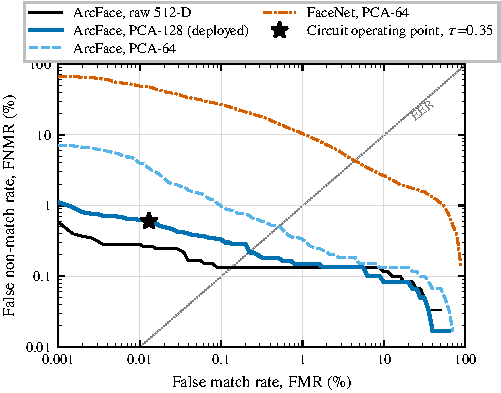
\includegraphics[width=\linewidth]{figures/fig_det.pdf}
    \caption{DET curves on LFW (6,000 genuine and 200,000 impostor test pairs, log axes). The star is the circuit's own decision at the deployed $\tau$ on integer coordinates; it lies on the floating-point PCA-128 curve.}
    \label{fig:det}
\end{figure}

\textbf{Face Encoding (RQ1):} Paired tests on the same pairs give three findings, and Fig.~\ref{fig:det} shows the full error trade-off: the deployed PCA-128 stays within a small factor of raw ArcFace's FNMR down to FMR $= 10^{-5}$, while PCA-64 and FaceNet fall well behind.
(i)~\emph{The embedding's rank decides what reduction costs:} 99\% of FaceNet's variance lies in 58 components, so PCA-64 is lossless for FaceNet (\nFacenetEer\%, equal to the mean-centred embedding; centring alone explains its gain over raw cosine, 0.37 points, CI [0.11, 0.64]). ArcFace needs 375 components, so every reduction costs accuracy and the dimension is a genuine trade-off.
(ii)~\emph{Deployed point, chosen without test data and against a stated attacker:} on validation identities we set $\tau$ so that a lookalike attacker screening $K = 100$ candidates succeeds at most 1\% of the time (\S\ref{subsec:eval_generalization}), and deploy the smallest dimension whose validation FRR at that $\tau$ is at most 1\%. PCA-112 misses (1.20\%); PCA-128 meets it (0.62\%, $\tau = 0.35$) and on the test pairs gives \nFrr\% FRR at \nFar\% zero-effort FAR. FaceNet meets the rule at no dimension. The usual zero-effort rule (FAR $\le 0.1\%$) would have selected PCA-96 at $\tau = 0.33$, whose EER is statistically indistinguishable from PCA-128's (0.05 points, CI [$-0.03$, 0.12]) but which the same attacker beats \nZeLookLfwHundred\% of the time (Fig.~\ref{fig:lookalike}): what separates the two is the FRR each needs to contain lookalikes, not the EER. PCA-160 is better still (0.05 points, CI [0.01, 0.13]) and costs \nOneSixtyExtra\% more constraints.
(iii)~\emph{The discriminant projection does not help at useful dimensions:} SOPQ is significantly worse than PCA on FaceNet (4.72\% at 64-D; 0.33 points, CI [0.08, 0.57]) and no better on ArcFace at any $d \ge 48$ (0.58\% vs.\ 0.52\% at 64-D, not significant; 0.32\% vs.\ 0.27\% at 96-D), beating PCA only at $d \le 32$. A DeepFace re-implementation of ArcFace reaches only \nDeepfaceEer\%, so the trained weights matter (Supplementary Material, Appendix~E).

\textbf{Constraint-Budget Sweep:} The face circuit grows by about \nPerDim{} constraints per output dimension (\nChunkedPerDim{} with per-coordinate hashing), mostly range checks: from \nFullCosSixteen{} at 16-D through \nFaceConstraints{} at 128-D to \nFullCosTwoFiftySix{} at 256-D, and raw 512-D ArcFace with no projection needs \nFullCosFiveTwelve{} (Fig.~\ref{fig:encoding_pareto}). Raw 512-D is thus feasible, but the voter's device stores the proving key and runs the prover for every ballot, and 512-D doubles the circuit and its FFT domain ($2^{16}$ vs.\ $2^{\nDomainExp}$). Measured with the same WASM prover (\path{bench_dim.sh}), witness generation and proving take \nRawProveMs~ms instead of \nDimProveMs~ms (+\nRawProveIncrease\%), the proving key grows from \nKeyMB{} to \nRawKeyMB~MB, and the prover needs \nRawExtraMemMB~MB more memory, all to reach \nRawEer\% instead of \nLfwEer\% EER. The rule therefore deploys the smallest dimension that meets both error targets. ArcFace's EER halves from 64-D to 96-D and flattens beyond 160-D; FaceNet's is flat beyond 64-D, as its rank predicts.

\begin{figure}[t]
    \centering
    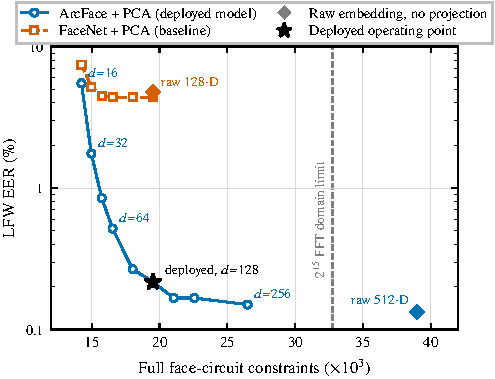
\includegraphics[width=\linewidth]{figures/fig_encoding_pareto.pdf}
    \caption{Accuracy vs.\ circuit cost as the PCA output dimension $d$ varies (16--256). Costs substitute measured sub-circuits into the compiled 128-D circuit; diamonds are the raw embeddings in-circuit. Past the dashed line the circuit needs a $2^{16}$ FFT domain, which doubles proving cost.}
    \label{fig:encoding_pareto}
\end{figure}

\subsection{Cross-Dataset Generalization and Lookalike Impostors}
\label{subsec:eval_generalization}

\textbf{Cross-Dataset (LFW vs.\ CelebA):} the PCA-128 fitted on LFW is applied without retraining to 2,000 randomly sampled CelebA identities (\nCelebaEmbedded{} of \nCelebaImages{} images embedded), yielding $\nCelebaEer\%$ EER [\nCelebaEerLo, \nCelebaEerHi] against LFW's $\nLfwEer\%$ (raw ArcFace \nCelebaRawEer\%, FaceNet PCA-64 \nFacenetCelebaEer\%). CelebA's low-resolution crops are harder for every model, and the projection fitted on LFW costs about half a point there. ArcFace was trained on WebFace600K; we did not verify that its identities are disjoint from LFW's and CelebA's.

\textbf{Age and Pose (CALFW, CPLFW):} On the 6,000-pair cross-age~\cite{Zheng2017CALFW} and cross-pose~\cite{Zheng2018CPLFW} protocols (CALFW impostors share gender and race), the deployed encoding reaches $\nCalfwEer\%$ [\nCalfwEerLo, \nCalfwEerHi] and $\nCplfwEer\%$ [\nCplfwEerLo, \nCplfwEerHi] EER (raw ArcFace \nCalfwRawEer\% and \nCplfwRawEer\%; the projection's cost is significant only under pose). At the deployed $\tau$, however, the circuit rejects \nCalfwFrr\% of genuine cross-age and \nCplfwFrr\% of cross-pose pairs, against \nFrr\% on LFW, while accepting \nCalfwFar\% and \nCplfwFar\% of impostors. Both sets reuse LFW identities; restricted to pairs whose identities are outside our training split, FRR is \nCalfwUnseenFrr\% and \nCplfwUnseenFrr\%. A threshold that contains lookalikes therefore rejects voters whose appearance has aged since enrollment or who are captured off-pose, so a deployment must re-enroll voters periodically and have the capture device enforce a frontal pose. Re-enrollment in turn needs leaf revocation, which the prototype lacks: NID deduplication blocks a second enrollment, and if allowed, the old leaf would stay in the append-only tree and give the voter a second nullifier. A per-election tree epoch, or a revocation list checked in \texttt{castVote}, would close this.

\begin{figure}[t]
    \centering
    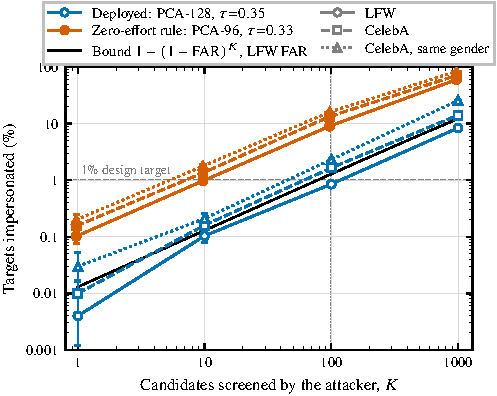
\includegraphics[width=\linewidth]{figures/fig_lookalike.pdf}
    \caption{Lookalike attack: share of targets impersonated by the best of $K$ screened candidates with one presentation, decided by the circuit (95\% Wilson intervals). Each target (2,300 LFW, 2,000 CelebA test identities) is enrolled from one image; the attacker ranks $K$ random other identities under the deployed ArcFace model, 20 pools per target. The bound uses the deployed point's LFW test FAR; CelebA's FAR is higher, and same-gender recruiting breaks the game's independence of candidates and target.}
    \label{fig:lookalike}
\end{figure}

\textbf{Lookalike Impostors:} The zero-effort FAR assumes a random impostor, but faces are public, so the realistic attacker, once it holds a stolen credential (\S\ref{sec:eligibility}), screens candidates' photos offline and recruits the best lookalike, and PAD does not stop a live lookalike. Fig.~\ref{fig:lookalike} measures this attack; success grows almost exactly as $K \cdot \mathsf{FAR}$ and stays below the LFW bound. Screening 100 candidates impersonates \nZeLookLfwHundred\% of LFW targets at the zero-effort rule's point but \nLookLfwHundred\% at the deployed point (\nLookCelebaHundred\% on CelebA, \nLookGenderHundred\% by gender), at a similar FRR. The CelebA rows, never used for selection, exceed the 1\% target, so a deployment should set $K$ and $\tau$ on data resembling its own capture conditions.

\subsection{Protocol Attack Suite, Demographic Fairness, and PAD Scope}
\label{subsec:eval_fairness_pad}

\begin{table}[t]
\caption{Protocol attack suite: each attack is a concrete witness or transaction submitted to the production chaincode (in-memory Fabric stub) with the deployed circuits. \emph{Base}: the design without the listed check; --: not applicable there. The \nAttacks{} attacks are these 27 plus A1 and A2 on the iris circuit and A5b (oversized coordinates, separate from A5's negated sample).}
\label{tab:attack_suite}
\centering
\footnotesize
\setlength{\tabcolsep}{2.5pt}
\renewcommand{\arraystretch}{0.9}
\begin{tabular}{@{}llp{2.85cm}cc@{}}
\toprule
\textbf{ID} & \textbf{Attack} & \textbf{Enforcing check} & \textbf{Base} & \textbf{Ours} \\
\midrule
A1 & Forged Merkle path & $d_\ell \in \{0,1\}$ constraint & \xmark & \cmark \\
A2 & Prover-chosen threshold & $\tau$ fixed in circuit & \xmark & \cmark \\
A3 & Fresh $\mathcal{E}_{\mathsf{id}}$ (re-vote) & chaincode $\mathcal{E}_{\mathsf{id}}$ check & \xmark & \cmark \\
A4 & Cross-ballot linkage & private biometric hash & \xmark & \cmark \\
A5 & Negated / oversized sample & sign + range checks & \xmark & \cmark \\
A6 & No live capture & in-circuit EdDSA attestation & \xmark & \cmark \\
A7 & Ciphertext substitution & $\mathsf{vb}$ public input & \xmark & \cmark \\
A8/A9 & Missing / invalid ciphertext & on-chain $\Sigma$-OR check & \xmark & \cmark \\
A10 & Phantom enrollment & registrar-only enrollment & \xmark & \cmark \\
A11 & Overvote & sum-to-one proof & -- & \cmark \\
A12 & Ballot copying & $\nu$ in Fiat--Shamir context & -- & \cmark \\
A13--16 & Foreign / replayed capture & signed message binding & -- & \cmark \\
A17 & One key opens a ballot & $t$-of-$n$ DKG key & \xmark & \cmark \\
A18--22 & Bad tally; late vote & closure, on-chain tally check & -- & \cmark \\
A23 & Inconsistent DKG share & complaint, $\mathsf{QUAL}$ & -- & \cmark \\
A24 & Carry-aliased template & range checks under packing & \xmark & \cmark \\
A25--27 & Enroll another's face & attested enrollment proof & \xmark & \cmark \\
\bottomrule
\end{tabular}
\end{table}

\textbf{Protocol Attack Suite:} Table~\ref{tab:attack_suite} turns each premise of Section~\ref{sec:security} into an executable attack (each circuit-level attack is run against both the face and the iris circuit, Supplementary Material, Appendix~D). Against the design without these checks, all 14 applicable attacks succeed (13 executed against the chaincode without the checks, A1--A10 with A1 and A2 on both circuits, and A25; A17 holds by construction, since its single tally key decrypts any ballot; for A24 a control shows that the aliased template has the victim's digest and passes the threshold against the attacker's face): an unregistered party could vote, any impostor could pass, one credential could vote without limit, a voter could enroll someone else's face, and the single tally key opened any ballot. With the checks, all \nAttacks{} are rejected while honest face and iris ballots and an honest 2-of-3 tally are accepted. A complaint disqualifies a dealer that sends an inconsistent share, and a false complaint is refused. An end-to-end client run confirms that the gateway never receives a key, salt, template, password or choice. \cmark{} = rejected.

\textbf{Demographic Fairness (Face, Gender):} On the same CelebA split used in \S\ref{subsec:eval_generalization} (2,000 identities, LFW-trained PCA applied without retraining), we partition identities by CelebA's \texttt{Male} attribute and measure EER of the deployed PCA-128 encoding within each subgroup: $\nMaleEer\%$ [\nMaleEerLo, \nMaleEerHi] on male-labeled identities (\nMaleIds) versus $\nFemaleEer\%$ [\nFemaleEerLo, \nFemaleEerHi] on female-labeled identities (\nFemaleIds). The gap of \nGenderGap{} points ($\nGenderRatio\times$) has non-overlapping CIs and is larger in relative terms than FaceNet's (\nFacenetMaleEer\% vs.\ \nFacenetFemaleEer\%). It is consistent with the higher female EER widely reported in face-verification fairness studies, and a deployment would need group-aware threshold or training mitigation. CelebA carries no ethnicity or skin-tone label, so that axis remains unevaluated.

\textbf{Presentation Attack Detection:} Sensor attestation (Theorem~\ref{thm:eligibility}) proves which registered device captured a sample, not that the sample is live; soundness against artefact presentations (photos, replays, masks) therefore rests on the device's PAD, which we treat as a capture-layer requirement and do not evaluate here. Live lookalikes are outside PAD's reach and are bounded only by $\tau$ (Fig.~\ref{fig:lookalike}).

\subsection{Circuit Footprint and Proving Latency}
\label{subsec:eval_circuit_benchmarks}

\begin{table}[t]
\centering
\caption{Face Circuit Artifacts and Per-Ballot Latency (20 ballots, $N = 1{,}000$; mean $\pm$ 95\% CI)}
\label{tab:combined_metrics}
\setlength{\tabcolsep}{4pt}
\renewcommand{\arraystretch}{1.1}
{\footnotesize
\begin{tabular}{@{}lr@{}}
\toprule
\textbf{Metric} & \textbf{Face (PCA-128)} \\
\midrule
R1CS constraints (\texttt{--O2}) & \nFaceConstraints \\
Proving key / proof & \nKeyMB\,MB / 128\,B \\
\midrule
\multicolumn{2}{@{}l}{\emph{Voter client (snarkjs WASM)}} \\
\quad Merkle paths (voter + device) & $\nMerkleMs \pm \nMerkleCi$\,ms \\
\quad Ballot encryption + proofs ($k{=}3$) & $\nEncryptMs \pm \nEncryptCi$\,ms \\
\quad Witness generation & $\nWitnessMs \pm \nWitnessCi$\,ms \\
\quad Groth16 proving & $\nProveMs \pm \nProveCi$\,ms \\
\quad \textbf{Client total} & $\mathbf{\nClientMs \pm \nClientCi}$\,ms \\
Capture device: attestation signing & $\nSignMs \pm \nSignCi$\,ms \\
\midrule
Groth16 verification & $\nVerifyMs \pm \nVerifyCi$\,ms \\
\textbf{Chaincode \texttt{castVote} (all checks)} & $\mathbf{\nCastVoteMs \pm \nCastVoteCi}$\,ms \\
\bottomrule
\end{tabular}}
\end{table}

\textbf{Latency (RQ2):} Groth16 proving dominates the client (\nProveShare\%). Packing puts the 128-D circuit's \nFaceConstraints{} constraints inside a $2^{\nDomainExp}$ FFT domain with room to spare, and the proving key at \nKeyMB~MB. Proving takes \nProveS~s, against \nIrisProveS~s for the \nIrisConstraints-constraint iris circuit on the same stack (Supplementary Material, Appendix~D). A complete ballot takes \nClientS~s with the WASM prover the browser client uses, on a desktop CPU.

\textbf{In a Real Browser:} We drove the unmodified React client in headless \nBrowserName{} with Playwright (\path{bench_browser.py}): \nBrowserVoters{} voters each enrolled from one LFW photo and voted with another photo of themselves. All ballots were accepted, an impostor presenting another face with the first voter's credential file and password was rejected by the circuit, a second vote by the chaincode, and the on-chain tally matched. In the browser, proving takes $\nBrowserProveMs \pm \nBrowserProveCi$~ms and a ballot $\nBrowserClientMs \pm \nBrowserClientCi$~ms (\nBrowserColdMs~ms for the first, which fetches the proving key); from the voter's click to commit, including capture attestation and Fabric's batching, takes \nBrowserSubmitS~s. On a phone (\nPhoneDevice, Safari), the same prover with the production keys takes $\nPhoneProveMs \pm \nPhoneProveCi$~ms for witness and proof (\nPhoneRatio$\times$ the desktop's \nDimProveMs~ms). A native prover would be faster but does not run in a browser, so we report the WASM figure. Sensor attestation adds \nAttestConstraints{} constraints, \nAttestShare\% of the face circuit, plus \nSignMs~ms of device signing.

\textbf{Euclidean Baseline Under the Same Stack:}\label{subsec:eval_baseline} Euclidean ZK matching (e.g.\ Mao et al.~\cite{Mao2023}) uses other proof systems, so we built a sound squared-Euclidean comparator in ours, with the same range checks and the equivalent constant threshold $\|\mathbf{a}-\mathbf{b}\|^2 \le (2-2\tau)\sigma^2$. On unit vectors it ranks pairs exactly as cosine does, and it saves only \nEuclidSave{} constraints at 128-D (\nEuclidConstraints{} vs.\ \nCosConstraints, \nEuclidSaveShare\% of the full circuit; Supplementary Material, Table~S3): range checks, \nRangePerCoord{} constraints per coordinate for either metric, dominate, so choosing $d$, not the metric, sets the cost.

\subsection{Scalability and Tallying}
\label{subsec:eval_scalability}

\textbf{Scaling with the Electorate (RQ2):}
Table~\ref{tab:scaling} sweeps $N$. Proving is constant, since the circuit always checks 20 levels. Chaincode verification is also constant (\nScaleCastMin--\nScaleCastMax~ms), because the chaincode maintains the voter-tree root incrementally at enrollment, so a vote needs only an $\mathcal{O}(1)$ root lookup rather than an $\mathcal{O}(NL)$ rebuild. The remaining $\mathcal{O}(N)$ cost is on the client, which builds its own Merkle path from the public commitment list (\nScalePathsTopS~s at $N = 2\times10^4$, extrapolating to $\sim$\nScalePathsMillionS~s at $10^6$). At national scale, paths would be served by an untrusted indexer, since the circuit verifies them against the on-chain root; we leave the privacy of path retrieval (e.g., fetching whole subtrees) to future work.

\begin{table}[t]
\centering
\caption{Scaling with Electorate Size $N$ (face, mean of 3) and Tally Size $M$}
\label{tab:scaling}
\setlength{\tabcolsep}{5pt}
{\footnotesize
\begin{tabular}{@{}rrrr@{}}
\toprule
$N$ & \textbf{Client paths} & \textbf{Proving} & \textbf{\texttt{castVote}} \\
\midrule
10 & \nScaleTenPathsMs\,ms & \nScaleTenProveMs\,ms & \nScaleTenCastMs\,ms \\
$10^3$ & \nScaleThousandPathsMs\,ms & \nScaleThousandProveMs\,ms & \nScaleThousandCastMs\,ms \\
$5\times10^3$ & \nScaleFiveThousandPathsMs\,ms & \nScaleFiveThousandProveMs\,ms & \nScaleFiveThousandCastMs\,ms \\
$2\times10^4$ & \nScaleTwentyThousandPathsMs\,ms & \nScaleTwentyThousandProveMs\,ms & \nScaleTwentyThousandCastMs\,ms \\
\midrule
$M$ & \textbf{Re-verify + agg.} & \textbf{2-of-3 decrypt} & \textbf{On-chain check} \\
\midrule
100 & \nTallyHundredVerifyS\,s & \nTallyHundredDecryptMs\,ms & \nTallyHundredPublishMs\,ms \\
$10^3$ & \nTallyThousandVerifyS\,s & \nTallyThousandDecryptMs\,ms & \nTallyThousandPublishMs\,ms \\
\midrule
\multicolumn{4}{@{}l}{\emph{Live network, submit to commit (\nFabVoters{} voters)}} \\
\multicolumn{3}{@{}l}{\texttt{castVote}: sequential / 10 in flight} & \nFabSeqS{} / \nFabConcS\,s \\
\multicolumn{3}{@{}l}{Throughput, 10 in flight (no MVCC conflict)} & \nFabTps\,tx/s \\
\multicolumn{3}{@{}l}{Registration / \texttt{publishTally}} & \nFabRegisterS{} / \nFabPublishS\,s \\
\multicolumn{3}{@{}l}{2-of-3 key generation (5 transactions)} & \nFabKeygenS\,s \\
\bottomrule
\end{tabular}}
\end{table}

\textbf{Tallying:} The trustees' software re-verifies every ballot's proofs before aggregating (\nTallyVerifyMs~ms per ballot, linear and trivially parallel). Two trustees then decrypt all totals with proofs in under 30~ms, since BSGS is $\mathcal{O}(\sqrt{M})$. The chaincode's own check, which recomputes the aggregates and verifies $t$ partial decryptions per option, takes \nTallyPublishS~s for 1,000 ballots. It runs in one transaction, so at $10^6$ ballots it would take about \nTallyMillionMin~minutes, far beyond Fabric's default chaincode timeout. A running aggregate under a single key would reintroduce the MVCC conflicts that per-vote keys avoid, so national scale needs sharded aggregates or batched sub-tallies, each verified in its own transaction; we have not implemented or measured this.

\textbf{Live Network:} We deployed the chaincode on Fabric's test network: two organizations with one peer each, CouchDB state, one Raft orderer, endorsement by both organizations, all on the benchmark host. We ran a 40-voter election through the gateway SDK, with every check in force. Sequentially, a vote takes \nFabSeqS~s from submission to commit. This is dominated by the orderer's batch timeout (the network's default cuts a block after 2~s or 10 transactions), not by the \nCastVoteMs~ms of chaincode work. With 10 votes in flight, blocks fill at once: each vote commits in \nFabConcS~s, and throughput is \nFabTps~votes/s with no MVCC conflict, because \texttt{castVote} writes only per-vote keys. All \nFabVoters{} votes were counted, and the on-chain tally check accepted the 2-of-3 decryption. At this rate $10^6$ votes would take about \nFabMillionH~hours. We did not try to saturate the network, and multi-host and WAN deployments remain to be measured.

\textbf{Comparison with Related Work:} Semaphore, MACI and World\,ID prove different statements on different hardware, so we do not tabulate their timings; our circuit proves their membership and nullifier statement plus an in-circuit match and capture attestation.


\section{Limitations and Future Work}
\label{sec:limitations}

\textbf{Lookalikes Bound the Concrete Guarantee.} The face is a second factor behind the credential. The deployed point contains an attacker who screens 100 candidates (\nLookLfwHundred\% success), not a larger one: screening 1,000, \nLookLfwThousand\% of LFW targets fall (Fig.~\ref{fig:lookalike}), and screening photos is cheap. The same threshold rejects \nCalfwFrr\% of genuine voters across an age gap and \nCplfwFrr\% across pose (\S\ref{subsec:eval_generalization}), and LFW, on which it was selected, is near saturation; a harder benchmark (e.g., IJB-C at FAR $= 10^{-4}$) remains to be run. Matching $K$ to a realistic attacker, and tuning $\tau$ on data resembling a deployment's enrollment interval and capture conditions, are the next steps.

\textbf{Linear Encodings Offer No Resistance to Witness Inversion.} If a template witness leaks from the client, a scenario outside our threat model that template protection is expected to address~\cite{ISO24745}, inverting the public PCA reconstructs an embedding that still verifies as the voter (EER \nInvEer\% vs.\ \nInvRawEer\% for genuine samples; Supplementary Material, Appendix~F). The standard mitigation, per-user secret rotation of the projection, is unattractive here: enforcing it in-circuit adds constraints, while a client-side-only rotation carries no cryptographic guarantee. Protection of the template therefore rests on keeping it in the voter's sealed credential.

Further limitations: (i)~\emph{Deployment Model and Capture Trust:} voting is at supervised kiosks; unsupervised remote voting would need hardware-attested phone keys. Receipt-freeness is not addressed (a voter can reveal the encryption randomness), and observed capture still requires physical isolation booths (\S\ref{sec:coercion}). Sensor attestation proves sample provenance, not liveness, so soundness additionally rests on the device's PAD, which we do not evaluate, and attested enrollment still needs the RA to check that the person at the kiosk holds the NID; (ii)~\emph{Registry:} the RA is trusted for eligibility; the prototype's $\mathsf{SHA256}(\text{NID})$ index is enumerable, and re-enrollment needs leaf revocation, which is not implemented (\S\ref{subsec:eval_generalization}); (iii)~\emph{Trustees and Tally:} the prototype runs the $n$ trustees in one process; separate deployment, the bias-free DKG of~\cite{Gennaro2007}, and recovery when fewer than $t$ trustees are online are not implemented, and the single-transaction on-chain tally check does not scale to national elections (\S\ref{subsec:eval_scalability}); (iv)~\emph{Fairness:} the gender gap is measured but not mitigated (\nMaleEer\% vs.\ \nFemaleEer\% EER, \S\ref{subsec:eval_fairness_pad}), while ethnicity and age group remain unevaluated pending suitably labeled datasets; the pretrained ArcFace weights are licensed for non-commercial research only; (v)~\emph{Iris:} the iris variant is near chance under classical segmentation (Supplementary Material, Appendix~D); (vi)~\emph{Deployment Measurements:} the live network ran on one host; saturation throughput and multi-host and WAN latency remain to be measured.

\section{Conclusions}
\label{sec:conclusions}
Zero-knowledge biometric eligibility fails at the constraints an honest prover never exercises. We named six such pitfalls (a free live witness, a prover-chosen threshold, unconstrained path bits, missing range checks, unbound public inputs and unattested enrollment) and showed each exploitable against a real chaincode: without its check, the attack succeeds; with the checks, all \nAttacks{} attacks are rejected. Closing them binds every live sample and every enrolled template to a registered kiosk in-circuit, and pins the threshold, the election and the ballot to the proof. Soundness also sets the cost: range checks, not the metric, dominate the comparator, and since they bound every coordinate, packing makes template hashing nearly free and shrinks the circuit by \nPackSave\%. Behind a stolen credential, a lookalike found by screening $K$ photos succeeds with probability at most $1-(1-\mathsf{FAR})^K$; selected on validation identities against $K = 100$, ArcFace PCA-128 at $\tau = 0.35$ (\nLfwEer\% EER on LFW, \nFrr\% FRR) holds that attacker to \nLookLfwHundred\%, against \nZeLookLfwHundred\% at the point the zero-effort rule selects, in \nFaceConstraints{} constraints. Voters prove in their browser in \nBrowserClientS~s; the chaincode enforces every check in \nCastVoteMs~ms per ballot, independent of electorate size, and verifies a $t$-of-$n$ threshold tally. The gateway, the RA, the kiosks and any $t-1$ trustees are outside the trust base for ballot privacy; for eligibility, the RA and the kiosk registry remain trusted.

\section*{Acknowledgment}
The authors used an AI assistant (Claude, Anthropic) to help audit the implementation, write analysis and benchmark scripts, draw Figs.~\ref{fig:architecture} and~\ref{fig:zkp_circuit}, and draft and edit text throughout the paper. The authors checked all content, results and references and take full responsibility for them.

\bibliographystyle{IEEEtran}
\bibliography{References}

\end{document}
